\chapter{Photon Reconstruction in \pandora}
\label{chap:Photon}

\chapterquote{When it is obvious that the goals cannot be reached, don't adjust the goals, adjust the action steps.}%
{Confucius, 551 BC - 479 BC}


%\section{Introduction}
Many aspects of the photon reconstruction are important. For example, the single photon energy resolution is necessary to reconstruct heavy particles using decay channels involving photons, such as tau lepton decay or \Ppizero decay. Another aspect of the photon reconstruction is the photon separation resolution, which is the measure of minimum spatially closeness of two resolved photons. The photon separation resolution, together with the photon completeness and purity, is crucial for a photon counting experiment, where the number of the photon is used as a physics quantity. The most recent example of such a photon-counting example, benefited from this photon reconstruction, is the  \HepProcess{\PHiggs \to \Pgamma \Pgamma} simulation study at \rootS{3} at the \CLIC \cite{Kacarevic:higgsToGammaGamma}.

Having an efficient photon reconstruction in a dense jet environment also improves the overall reconstruction. As the particle flow approach to the calorimetry aims to reconstruct each individual particle, by assigning correct calorimeter hits to photons, assigning the remaining hits to the tracks for charged particles becomes an easier problem. Hence the track-cluster association can be achieved with fewer mistakes, and the jet energy resolution improves.

%Since the essential part of the particle flow reconstruction is the track-cluster association,  a high-performance photon reconstruction thus leads to a reduced-density environment for charged-particle reconstruction, which in return improves the
This chapter discusses a number of photon reconstruction algorithms within the \pandora framework, followed by the performances of these algorithms. Part of this chapter has been published in a conference proceeding \cite{Xu:2016rcz}.

%The ability to reconstruct photons in a collider experiment is important.




%Photon reconstruction is an important part of \pandora reconstruction. A good photon reconstruction should provide a good single photon completeness and purity, as well as a good photon separation resolution. For many physics processes, heavy particles decaying into photons, such as \Ptau lepton and \Ppizero. Photon reconstruction is crucial for reconstructing these heavy particles.

%The photon reconstruction presented in this chapter has improved the photon reconstruction completeness by reducing the fragments. The photon separation resolution has  also been improved. This work has been published in a conference proceeding \cite{Xu:2016rcz}. The improved  photon reconstruction has benefited many physics analyses involving photons. The most recent example is the  \HepProcess{\PHiggs \to \Pgamma \Pgamma} analysis at \rootS{3} at \CLIC \cite{Kacarevic:higgsToGammaGamma}.

%This set of photon related algorithms have been incorporated into the default reconstruction chain in \pandora. The \CLIC simulation studies have benefited from the improved photon reconstructions in various physics process, such as  \HepProcess{ \PHiggs \to \Pgamma \Pgamma}.

\begin{comment}
Since the discovery of a particle consistent with being the SM Higgs boson in LHC at 2012 \cite{Aad:2012tfa,Chatrchyan:2012ufa}, our understanding of Standard Model has improved greatly. Yet limited by the underlying QCD interaction from proton-anti-proton collision, one has great difficulty to measure the properties of the Higgs precisely. Next generation electron-positron linear collider could hopefully make precision measurements of the Higgs sector and the Top quark sector \cite{Abramowicz:2013tzc}.

The leading candidates for next generation electron-positron linear collider are the International Linear Collider (ILC) \cite{Brau:2007zza}, and the Compact Linear Collider (CLIC) \cite{Linssen:2012hp}. The ILC has developed two detector models, namely the International Large Detector (ILD) \cite{Abe:2010aa} and the Silicon Detector (SiD) \cite{Aihara:2010zz}. The CLIC has developed two slightly modified detector models based on ILD and SiD \cite{Linssen:2012hp}. One key common feature of these next generation electron-positron linear colliders is the high granular calorimeter, which provides a great spatial resolution at the cost of the energy resolution. Particle flow algorithms (PFA) benefit from the spatial resolution from calorimeters, together with tracking information, to provide excellent a jet energy resolution. PandoraPFA, the most complicated and the best performing one, provides a jet energy resolution of less than 3.5\%, which is required for W/Z separation \cite{Thomson:2009rp,Marshall:2013bda}.

\begin{figure}[tbph]
\centering
{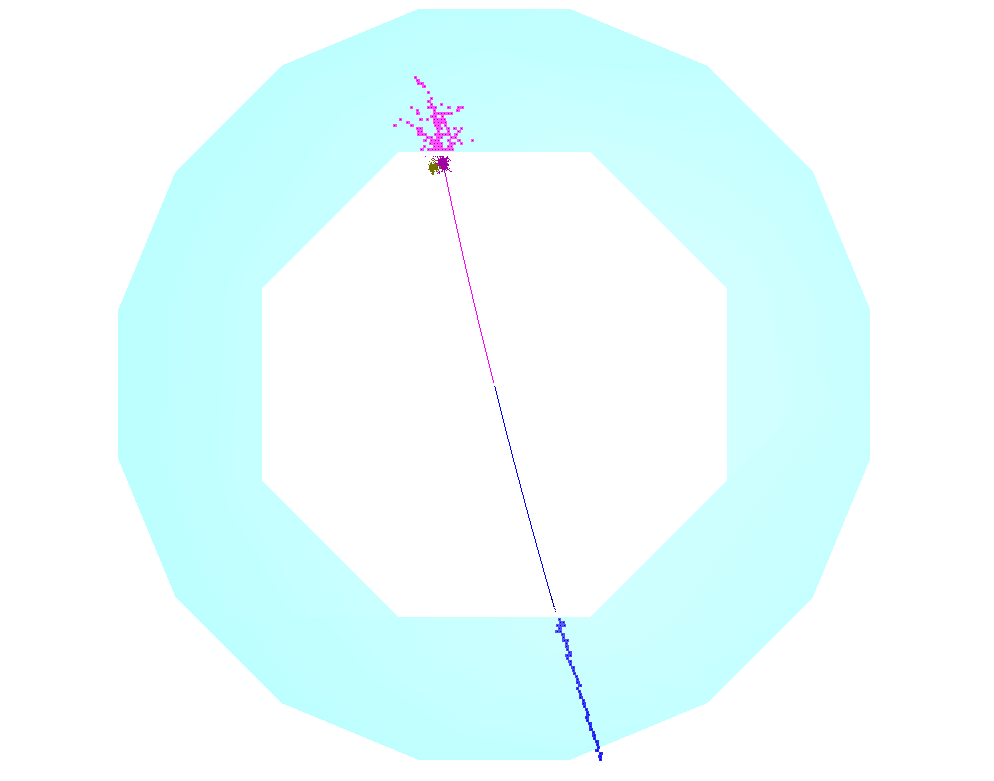
\includegraphics[width=0.5\textwidth]{images/tautauMod}}%

\caption{An event display of a simulated $\Pem\Pep\to \Ptauon\APtauon$ event. The blue region is the cross section of the Electromagnetic Calorimeter barrel region. The top $\Ptau$ decays into a charged $\Ppi$, two photons and neutrinos. The bottom $\Ptau$ decays into a muon and neutrinos.}
\label{fig:Tautau}
\end{figure}

Photon reconstruction is an important part of particle reconstruction. For many physics processes involving particles decaying into photons, such as $\Ptau$ lepton and $\Ppizero$, a good photon reconstruction, which provides a good single photon completeness and purity, as well as a good photon separation resolution, is crucial for reconstructing these particles.

\end{comment}

%\section{Electromagnetic shower}

\section{Overview of photon reconstruction in \pandora}

\pandora is a multi-algorithm pattern recognition software package for the event reconstruction and an implementation of the particle flow approach to calorimetry. A detailed discussion of the \pandora and the main steps of the \pandora event reconstruction can be found in \Section{sec:pandoraPandoraPFA}. As the \pandora reconstruction aims to reconstruction individual particles, photons are reconstructed with \pandora. The multi-algorithm approach of the \pandora allows each algorithm deals with a particular issue in the reconstruction. In the context of the photon reconstruction, there are four five algorithms developed to tackle different issues in the photon reconstruction.

The most important photon algorithm is the \PhotonReconstruction algorithm. It carefully reconstruct photons from calorimeter hits in the \ECAL, including forming a photon candidate and applying a photon ID test,
with special treatments for photons close to charged particles. This algorithm is implemented at the early stage of the reconstruction (see \Section{sec:particleID}), aiming to provide a clean environment for the subsequent charged-particle reconstruction.


Three algorithms are designed remove photon fragments at a later stage in the reconstruction. Two photon fragment removal algorithms merge fragments in the \ECAL, and one algorithm merges fragments in the \HCAL. These algorithms improve the single photon energy resolution.

The last photon algorithm is a photon splitting algorithm. The algorithm seeks to separate accidently merged photons, which helps photon separation resolution.

These algorithms together form the photon reconstruction in the \pandora. This chapter will first introduce the photon-induced electromagnetic shower in a calorimeter, followed by the description of each algorithm. The performance of the photon reconstruction will be provided in the last part of the chapter.

\begin{comment}
\pandora provides a framework for particle reconstruction \cite{Marshall:2015rfa}, as described in \Section{sec:pandoraPandoraPFA}. In the linear collider user case, it has a vast library of algorithms developed over years by many people. Each algorithm addresses one topological issue in the particle reconstruction. The essential part of the \pandora is track-cluster association  to find the best track-cluster pair, and re-clustering to find the best cluster consistent with the track. Other algorithms that identifies trackless clusters, such as muon clusters or photon clusters, would provide a cleaner environment for the track-cluster association, hence improving the jet energy resolution.

Photon identification in \pandora has two main mechanisms. The basic mechanism performs photon identification at the last step of the reconstruction  (see \Section{sec:pandoraPFOcreation}). The second more sophisticated photon identification is performed at an early stage of the reconstruction  (see \Section{sec:particleID}). The second algorithm identifies photon electromagnetic shower cores carefully in a dense jet environment. By removing photons from the environment, fewer calorimeters hits are left for charged particle reconstruction. Hence the overall reconstruction improves.

The \PhotonReconstruction algorithm in \pandora version 1 improves jet energy resolution by correctly identifying photon electromagnetic shower cores and leaving a cleaner environment for the track-cluster association. However, peripheral calorimeter hits to the shower cores may be reconstructed as separate particles (fragments). This lowers the reconstructed photon completeness and makes the number of reconstructed photons a less useful physical quantity. Also, the algorithm in \pandora version 1 leaves rooms for improvement of photon separation resolution.

This chapter presents a solution to photon reconstruction issues. The newly introduced algorithms reduces photon fragments and improves the photon separation resolution.

%Some part of the work has been published in a conference proceeding \cite{Xu:2016rcz}.

Firstly an overview of electromagnetic showers is presented. The \PhotonReconstruction algorithm will be described next, followed by fragment removal algorithms and photon splitting algorithms. This chapter will end with a discussion on performances of these photon related algorithms,  including comparisons with the previous photon algorithm.
%Algorithms related to photon reconstruction, fragmental removal and photon splitting, which are written or introduced by authors, will be discussed below.
\end{comment}

%The testing simulated data in this paper are generated either by WHIZARD \cite{whizard} or by the simple HepEvt generator. Events are simulated with GEANT4 \cite{Agostinelli:2002hh} in MOKKA \cite{MoradeFreitas:2002kj}. Jet fragmentation was performed with PYTHIA \cite{Sjostrand:1995iq} and the particle reconstruction was done by PandoraPFA \cite{Marshall:2015rfa} in MARLIN reconstruction framework \cite{Gaede:2006pj}, in ILD\_o1\_v6 detector model. The iLCSoft v17-01-07 was used. Different versions of PandoraPFA were used for the comparison purpose.

\section{Electromagnetic shower}
\label{sec:photonEMshower}
An electromagnetic (EM) shower refers to the pair production and bremsstrahlung when a high energy photon or electron passing though a thick absorber. The properties of the EM shower is the basis of forming photon candidates, photon ID test, and photon separation.

The pair production and bremsstrahlung generate many low energy photons and electrons, producing a shower-like  structure, hence the name EM shower. Two suitable length scales to describe the EM shower are the radiation length and the \RM. The radiation length of a material is used to describe the longitudinal shower profile, defined as the mean distance travelled where an electron loses its energy by a factor of $1/e$ via bremsstrahlung. It is also defined as the mean free path  for pair production by a high energy photon\cite{segre1977nuclei}. The \RM of a material is a suitable length describe the transverse shower profile.

\begin{figure}[tbph]
\centering
{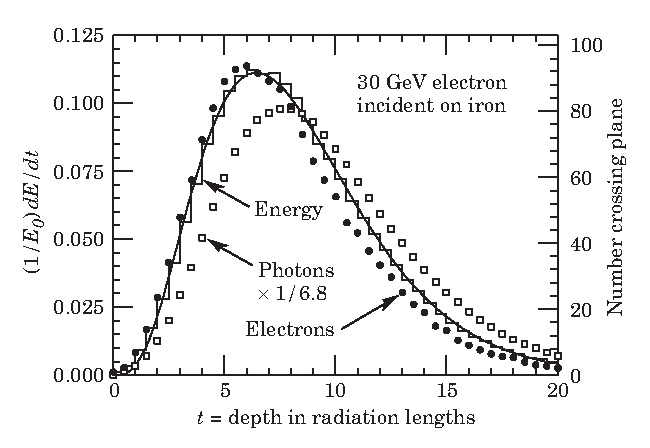
\includegraphics[width=0.65\textwidth]{photon/EMlong}}
\caption[Simulated longitudinal electromagnetic shower profile as a function of depth for electrons and photons.]
{An EGS4 simulation of a 30\,GeV electron-induced electromagnetic shower in iron. The histogram shows fractional energy deposition as a function of radiation lengths, and the curve is a gamma-function fit to the distribution. Circles and squares are the number of electrons and photons respectively with total energy greater than 1.5\,MeV crossing planes with scale on right. Plot is taken from \cite{Agashe:2014kda}.}
\label{fig:photonEMlongProfile}
\end{figure}

\FIGURE{fig:photonEMlongProfile} shows the simulated longitudinal electromagnetic shower profiles as a function of radiation length for electrons and photons. The mean EM longitudinal shower profile can be described by the following function \cite{Longo:1975wb} :
\begin{equation}
\frac{dE}{dt} = E_0 b \frac{\parenths{bt}^{a-1}e^{-bt}}{\Gamma(a)},
\label{eq:photonEMshower}
\end{equation}
where $t$ is the number of radiation lengths; $a$ and $b$ are free parameters; and $E_0$ is the shower energy. $b$ varies slightly with material but it is sufficient to use $b = 0.5$ for the purpose of photon reconstruction. $a$ is calculated to be:
\begin{equation}
a = 1.25 + 0.5ln\left(\frac{E_0}{E_c}\right),
\end{equation}
where $E_c$ is the critical energy. This parametrisation should only be used to describe an average behaviour of the EM shower, as the fluctuation is important.

%For the photon identification, the longitudinal shower profile is compared with \Equation{eq:photonEMshower}.

The transverse shower profile can be described as  a narrow cone widening as the shower develops. 90\% of the energy  is contained in a fiducial cylinder with a radius of one \RM. Transverse profile is often represented by a sum of two Gaussian function. The Gaussian nature of the transverse profile allows the separation of two EM showers using a two dimensional peak finding algorithm.

\section{\PhotonReconstruction algorithm}
\label{sec:photonRecostrcution}


The \PhotonReconstruction algorithm is a photon reconstruction and  identification algorithm at the early stage of the reconstruction. It correspondes to ``Particle ID'' stage in \Section{sec:particleID} of the \pandora reconstruction chain.  Main steps of the \PhotonReconstruction algorithm, shown in \Figure{fig:photonPhotonRecoFlow}, are:  coarsely forming photon clusters; finding photon candidates; photon ID test; and optional fragment removals. Finding photon candidates uses the transverse shower profile information, which requires a  two dimensional peak finding algorithm, further explained in \Section{sec:peakFinding}. The photon ID test involves a multi dimensional likelihood classifier, which is described in \Section{sec:photonLikelihood}. The optional fragment removal algorithm shares a common code base case class with another photon fragment removal algorithm. Hence two photon fragment removal algorithms are discussed together in \Section{sec:photonFragRemoval}.

\begin{figure}[tbph]
\centering
{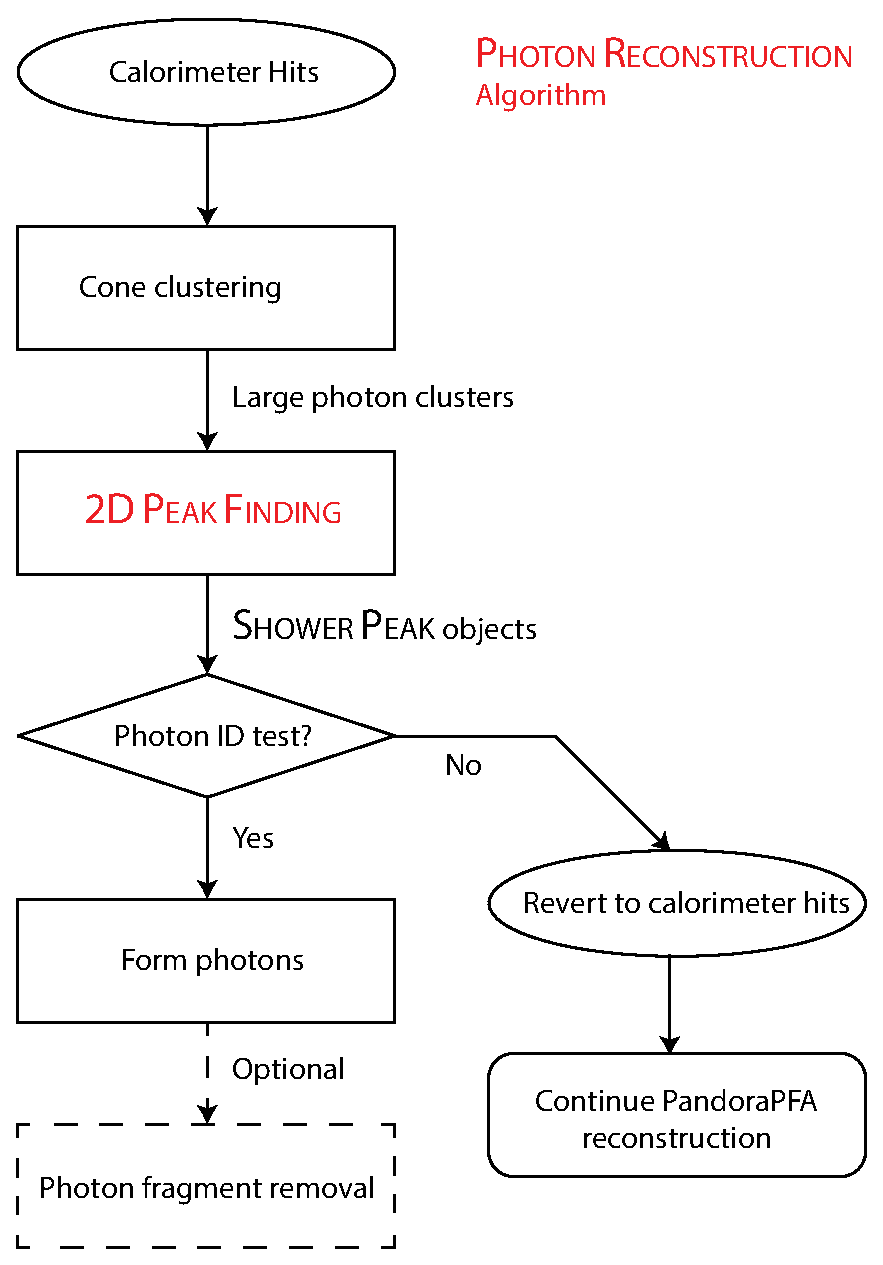
\includegraphics[width=0.45\textwidth]{photon/photonRecoFlow}}
\caption[A flow diagram of the \PhotonReconstruction algorithm.]
{A flow diagram showing main steps in the \PhotonReconstruction algorithm.}
\label{fig:photonPhotonRecoFlow}
\end{figure}


\subsection{Form photon clusters}

The inputs of the \PhotonReconstruction algorithm are calorimeter hits in the \ECAL, that have not been used in previous algorithms. For example, muon reconstruction algorithms will form muons and remove calorimeter hits associated with muons from the reconstruction. The \PhotonReconstruction algorithm finds large potential photon clusters in the \ECAL. The clusters are formed such that a photon would not be split into two clusters, but one cluster may contain multiple photons. For simplicity, the algorithm opts to reuse  the cone clustering algorithm (see \Section{sec:pandoraConeCluster}) provided inside \pandora to find large clusters.  Since the target for reconstruction is neutral electromagnetic shower in the \ECAL, the cone cluster algorithm is set to use high energy calorimeter hits as initial seeds.  %The parameters for the cone clustering are such that  forming large clusters is preferred.

\subsection{Find photon candidates}
\label{sec:photonCandiate}

The next stage is to refine large photon clusters into smaller photon candidates. The aim of the refined photon candidate is that each candidate should contain calorimeter hits from one photon only. The method for refining clusters is to split a three-dimensional cluster into several smaller clusters. The three-dimensional splitting problem is hard. Therefore, a translation is needed to map the three-dimensional problem to a more manageable two-dimensional problem. The translation relies on the  transverse distribution of characteristic EM showers, which is characterised by a narrow cone, widening while the shower develops. Along the direction of the photon, an  EM shower can be modelled as a dense shower core with peripheral hits around the core. When the energy deposition is projected on to a plane, the EM shower core would appear as a mountain-like structure in the plane. One example  a large photon cluster projected on to a two dimensional plane, where two EM showers are identified, is shown in \FIGURE{fig:photonPeakFinding}. Hence, by identifying a peak in the two dimensional plane, an EM shower core is identified.  Thus the three-dimensional cluster splitting problem is mapped to a two-dimensional peak finding problem with the projection translation.

%the energy deposition projection of two photons candidates. U and V axis are two arbitrary orthogonal axis in the transverse plane perpendicular to the direction of photons. Z axis shows the sum of the calorimeter hit energy in GeV. The bin size corresponds to the square \ECAL cell size.


%To reduce the problem of splitting a three dimensional clusters (a collection of hits) into a manageable two dimensional problem.

%The large photon clusters are split into smaller photon candidates, using two-dimensional shower profiles. The candidates close to a track projection are deemed as non-photons. Identifying photon candidates within a large photon cluster relies on the characteristic electromagnetic showers, in particular the transverse distribution. A energetic photon or electron hits the absorber layers of the \ECAL, it initiates an electromagnetic shower, where electron pair production and bremsstrahlung produce more low-energy photons and electrons. The transverse distribution is characterised by a narrow cone, widening while the shower develops.

%To view the transverse shower distribution, a two-dimensional energy deposition projection is constructed in the plane perpendicular to the direction of the cluster. \Figure{fig:photonPeakFinding} shows the energy deposition projection of two photons candidates. U and V axis are two arbitrary orthogonal axis in the transverse plane perpendicular to the direction of photons. Z axis shows the sum of the calorimeter hit energy in GeV. The bin size corresponds to the square \ECAL cell size.

\begin{figure}[tbph]
\centering
{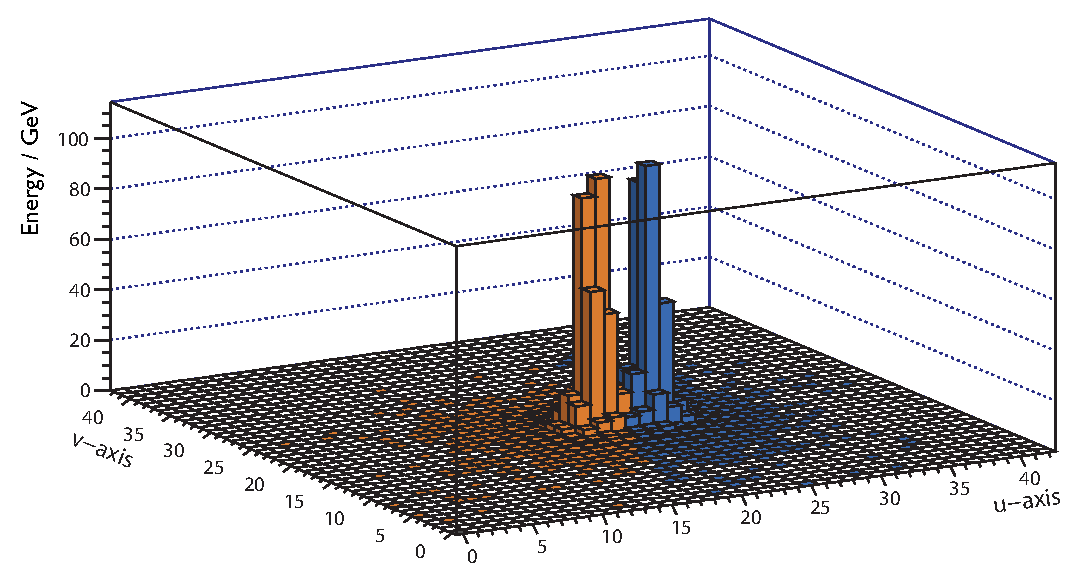
\includegraphics[width=0.5\textwidth]{photon/peakFindingMod}}
\caption[Example of projecting a large photon clusters containing two photons.]
{Two 500\,GeV photons (yellow and blue), just resolved in a transverse plane orthogonal to the direction of the flight  by projecting their energy deposition in the \ECAL. U and V are orthogonal axes in units of the \ECAL cell sizes. Z axis is the sum of the calorimeter hit energy in GeV.}
\label{fig:photonPeakFinding}
\end{figure}

By using the two-dimensional energy deposition projection, separating photons translates to separating peaks in the projection. Therefore a high-performance two dimensional peak finding algorithm is the key to identify photon candidates within a photon cluster. Due the complexity of the projection, a separate peak finding algorithm is developed and discussed in \Section{sec:peakFinding}. The output of the two dimensional peak finding is a collection of \ShowerPeak objects. Each \ShowerPeak object, which is used as the input for the next step, corresponds to a photon candidate and associated contains calorimeter.

\subsection{Photon ID test}
\label{sec:photonIDtest}

This step applies the photon ID test on the photon cluster, which is stored in the form of a \ShowerPeak object. The photon ID test uses  a multidimensional likelihood classifier, which needs to be trained before applying. A set of variables, which exploit features of electromagnetic showers, are used. The response from the classifier determines if a photon cluster is a photon. If it is a photon, the cluster would be tagged as a photon and the cluster does not participate in the event reconstruction until at the fragment removal stage after the charged particle reconstruction. If the cluster is not a photon, the cluster will be reverted to associated calorimeter hits. The hits will be passed on to the next stage of the reconstruction (see \Figure{fig:photonPhotonRecoFlow}). Because the multidimensional likelihood classifier is complicated, the classifier is discussed in \Section{sec:photonLikelihood}.



\subsection{Photon Fragment removal}
\label{sec:photonRecoFragRemoval}

The  photon fragment removal algorithm aims to merge small photon fragment to identified photons. The algorithm is optional as it is not run by default settings. Since this step shares the same logic as the fragment removal algorithm in \Section{sec:photonFragRemoval}, two algorithms are discussed togethers in a later \Section{sec:photonFragRemoval}.

%only differing in the cut-off values for merging metrics, this step be discussed in \Section{}.

This step marks the end of the photon reconstruction algorithm. The output are a collection of reconstructed photons, separated from non-photon calorimeter hits. These photons do not participate in the event reconstruction until at the fragment removal stage (see \Section{sec:pandoraFragmentRemoval}) after the charged particle reconstruction.
%The candidate passed the test will be kept in a separate container for photons only

\section{Two dimensional peak finding algorithm for photon candidate}
\label{sec:peakFinding}

As discussed in \Section{sec:photonCandiate}, identifying photon candidates inside a cluster is translated to identifying peaks in a two dimensional plane, with the use of the two dimensional peak finding algorithm ( \peakFinding algorithm). An example of two photons resolved in a two dimensional plane is shown in the \Figure{fig:photonPeakFinding}. The \peakFinding algorithm aims to correctly identify peak positions in a two dimensional histogram and associate calorimeter hits.

There are two variants of the \peakFinding algorithm: the neutral cluster variant and the charged cluster variant. The base algorithm treats all clusters as potential photon clusters, which is referred to as the neutral cluster variant. A flow chart of the main steps of the  neutral cluster variant is shown in \Figure{fig:photonPeakFindingFlowNeutral}. Since charged hadrons would deposit tracks in the tracking system, extra care is taken when a cluster is close to the projection of the track in the front of the \ECAL (see \Section{sec:photon2Dtrack}). The neutral cluster variant is described first, followed by the modification for charged cluster variant. The main steps of the charged cluster variant are shown in \Figure{fig:photonPeakFindingFlow}.

\begin{figure}[tbph]
\centering
{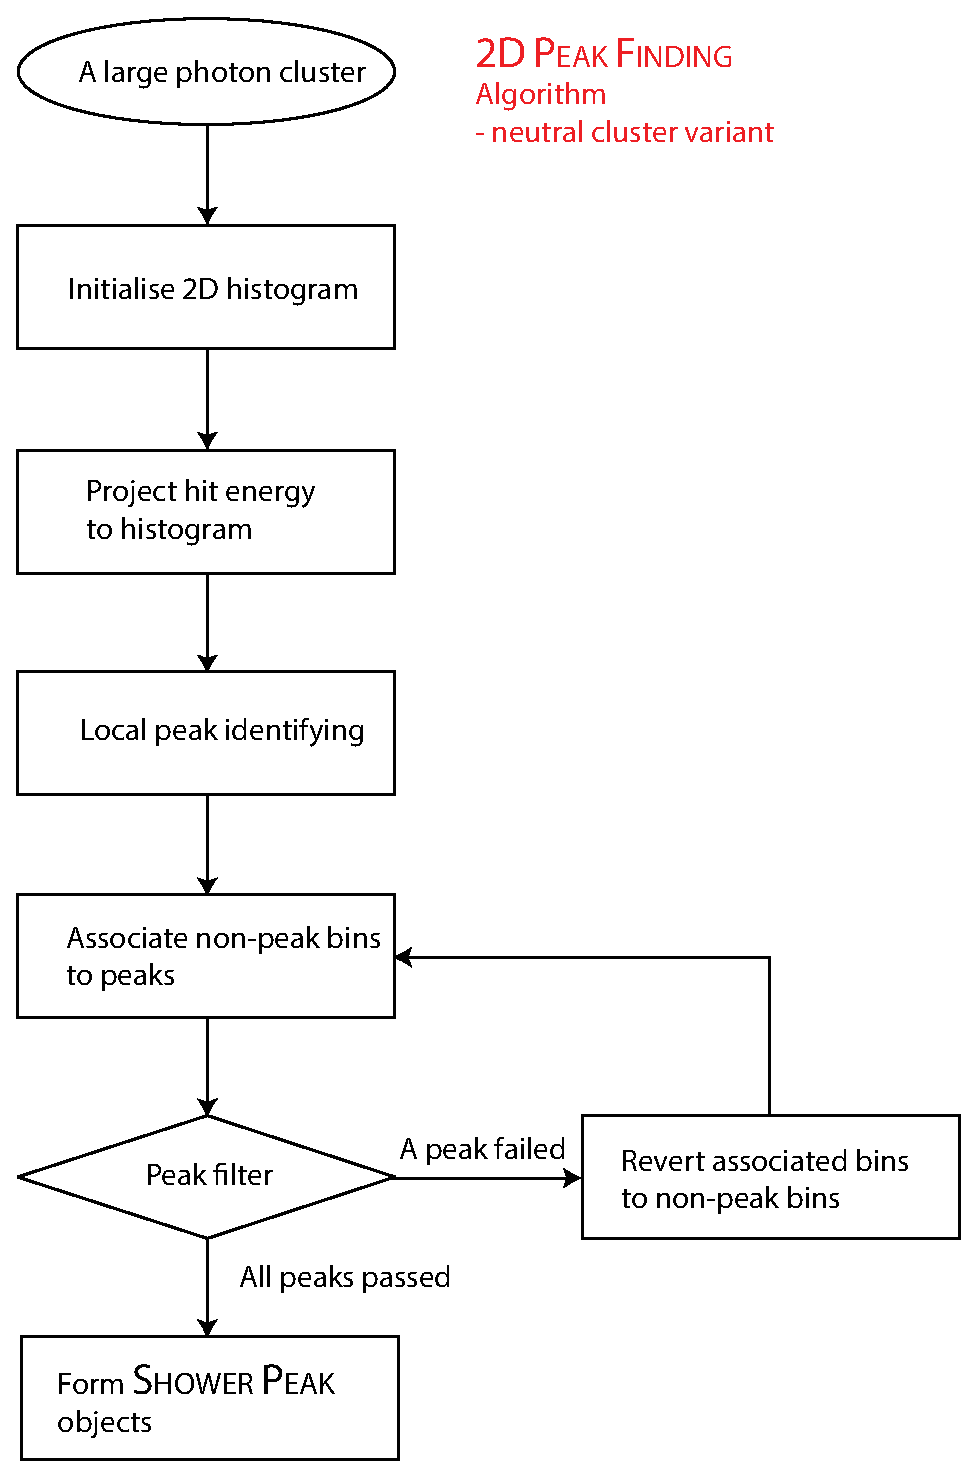
\includegraphics[width=0.5\textwidth]{photon/2DpeakFinding}}
\caption[Flow chart for \peakFinding algorithm neutral cluster variant.]
{Flow chart showing main steps in the  neutral cluster variant of \peakFinding algorithm.}
\label{fig:photonPeakFindingFlowNeutral}
\end{figure}

\subsection{Initialise the  two dimensional histogram}

This step initialise a two dimensional (2D) histogram to host the projection of the energy deposition of the photon cluster. For the best resolving power between photons, the projection direction is chosen to be the direction of the cluster. Two axes of the two dimensional histogram are chosen such that axes and the direction of the cluster form an orthogonal bases in the three dimensional space.

%The axes are labelled as  U and V axis in \Figure{fig:photonPeakFinding}.



\subsection{Project hit energy to histogram}

This step projects positions of the calorimeter hits, which are associated with the photon cluster, onto the 2D histogram initialised in the previous step. For a finite sized 2D histogram, the projection is chosen such that the cluster centroid position is at the centre of the histogram. The bin size along both axes corresponds to one \ECAL square cell length. The relative distance between the calorimeter hit position and the cluster centroid position is converted into a distance vector. The distance vector is subsequently projected onto the histogram using the scalar product with the axes vectors. The distance vector, $\vec{s_{i}}$, of a hit $i$ is obtained by:
\begin{equation}
\vec{s_{i}} = \frac{\vec{a_{i}} -  \vec{\angles{a}}}{d_{cell}},
\end{equation}
where $\vec{a}$ is the three dimensional position of the hit $i$;  $\vec{\angles{a}}$ is the centroid position of cluster $a$; and $d_{cell}$ is the  \ECAL square cell length.

The projected position on the 2D histogram is binned at integer intervals. The bin height is the sum of the energies associated with the calorimeter hit fall in that particular bin.

%The issue with the histogram size being finite is discussed in \Section{sec:photonPeakFindingInclusive}.

\subsection{Local peak identifying}

This step identifies all local peaks in the 2D histogram. For example, in \Figure{fig:photonPeakFinding}, there are clearly two peaks, both colour coded. A local peak is defined as a bin where its height is above all eight neighbouring bins. The 2D histogram is scanned linearly to identify all peaks. %Hence the processing time is $O\left(N^2\right)$, where $N$ is number of bins in one axis.

\subsection{Associate non-peak bins to peaks}

Having tagged all local peaks, this step associates non-peak bins to peaks based on the energy of the peak and the distance of the non-peak bin to the peak bin. The energy dependence is needed as the transverse EM shower width increases with the increase of the energy. The distance dependence is because the EM showers have dense shower cores.

After all local peak bins are found, non-peak bins are associated to a peak bin. The peak bin is chosen by minimising the metric
\begin{equation}
\min_{i}\frac{d_{i}}{\sqrt{E_{i}}}
\end{equation}
where $d_{i}$ is the Euclidean distance between a non-peak bin and a  peak bin $i$ on the histogram, and $E_{i}$ is the height of the peak bin $i$. The metric is iterated over all peak bins for each non-peak bin. Alternative metrics provided in the algorithm include $d_{i}$, $\frac{d_{i}}{{E_{i}}}$, and $\frac{d_{i}}{{E_{i}^2}}$. The default metric is chosen due to a good balance between distance and energy of the peak.

%And EM shower is typically narrow transversely.

\subsection{Peak filtering}

The performance of the two dimensional peaking finding algorithm is improved by clever programming and physics arguments. For a given two dimensional histogram, such as the one in \Figure{fig:photonPeakFinding}, major peaks most likely correspond to physical photons, while the minor peaks more likely come from fluctuations in the energy deposition. To select major peaks, every time after all non-peak bins are associated with peak bins, minor peaks with fewer than three bins associated (including the peak bin) are discarded. These discarded bins are re-associated with other peak bins. This iterative process stops when all peak bins have at least three bins associated.

The peak filtering step also allows bins with height below a critical value to not participate in the peak finding. The default value is set such that only empty bins are not used.

The \ShowerPeak  object is created, which contains one peak bin and associated non-peak bins. The associated calorimeter hits with the bins are attached to the \ShowerPeak object as well. If multiple peaks are identified in a cluster, multiple \ShowerPeak objects are created as outputs.

This marks the end of the neutral clusters variant of the \PhotonReconstruction algorithm, outlined in \Figure{fig:photonPeakFindingFlowNeutral}. The  \ShowerPeak object is also referred to as the photon candidate.

\subsection{Candidate close to track projection}
\label{sec:photon2Dtrack}
If a cluster or a photon candidate is close to the projection of the track in the front of the \ECAL, it is more likely that the cluster or the candidate is a charged hadron. Misidentifying a charged hadron as a photon leads to significant degradation in reconstruction performance. However, if a photon next to a charged hadron is carefully reconstructed, the overall reconstruction is improved. Hence this step aims to carefully identifies photon candidates next to charged hadrons, by using track information and features of EM showers, such as electromagnetic shower typically starting in first few layers of the \ECAL with direction of the EM shower largely unchanged.

\begin{figure}[tbph]
\centering
{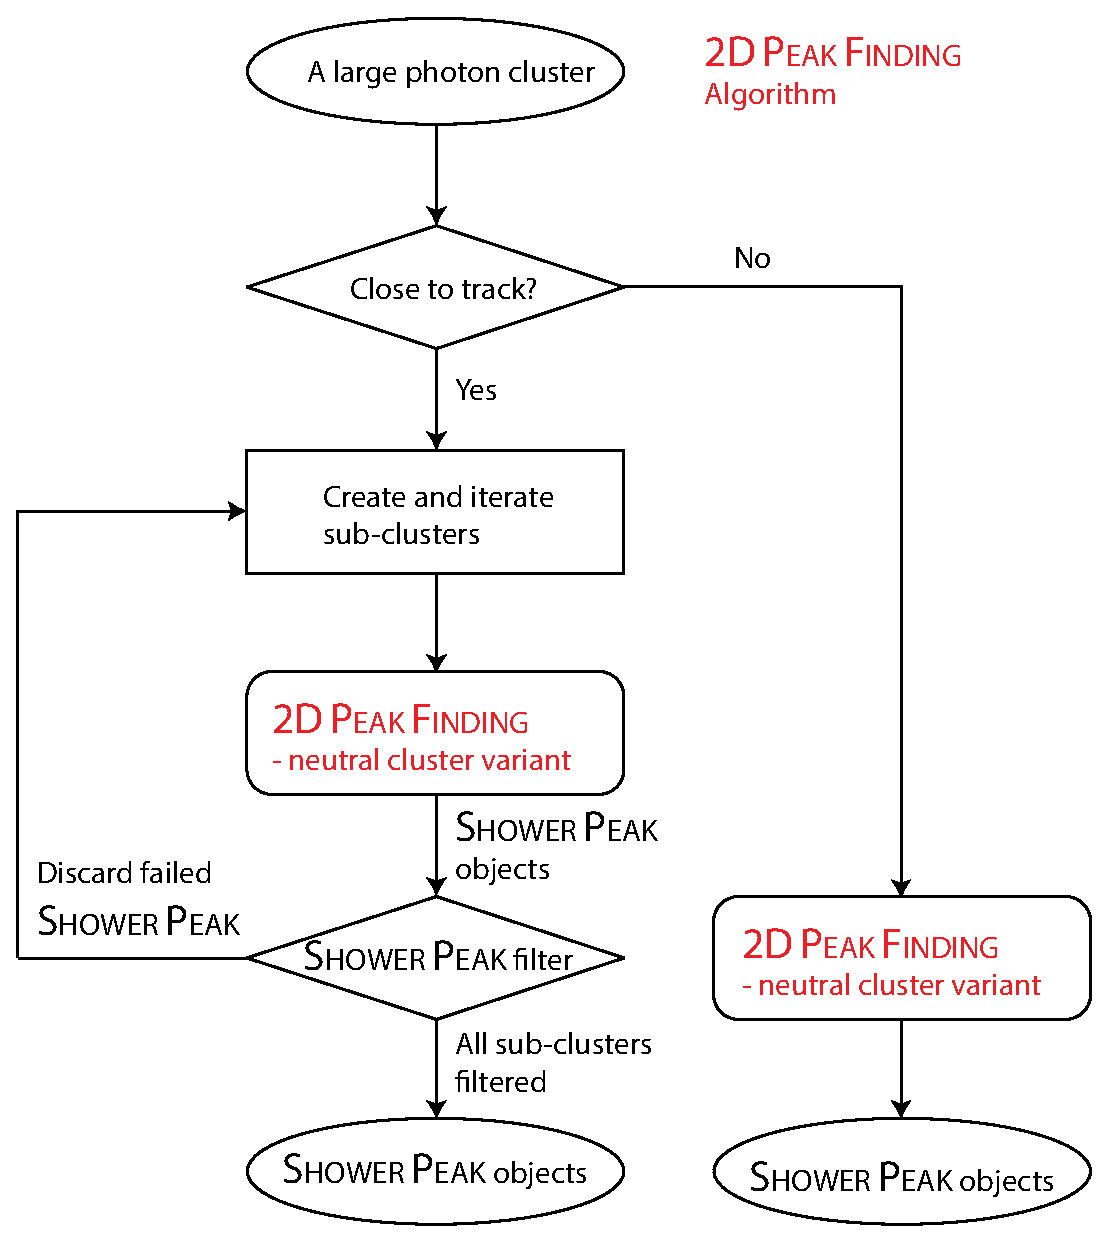
\includegraphics[width=0.7\textwidth]{photon/2DpeakFindingTrack}}
\caption[Flow chart for \peakFinding algorithm.]
{Flow chart showing main steps in the  \peakFinding algorithm, including the charged cluster variant.}
\label{fig:photonPeakFindingFlow}
\end{figure}

\FIGURE{fig:photonPeakFindingFlow} shows the main steps in the full \peakFinding algorithm, including the treatment to clusters close to tracks. The "Close to track" step determine if a cluster is close to a track. If a cluster is less than 3\,mm from the closest track projection, it is treated as a potentially charged cluster. The "Create and iterate sub-clusters" performs the following. The \ECAL is sliced longitudinally to help identify photon candidates. For example, the default three slices will result in three \ECAL fiducial spaces, which cover spaces from the front of the \ECAL to a third, two thirds and the back of the \ECAL, respectively. Three sub-clusters contained in each fiducial space are created. The neutral cluster variant of the  \peakFinding algorithm is then repeated for each sub-cluster. The \ShowerPeak objects created from each sub-cluster undergo the "\ShowerPeak filter" step. All peaks and associated \ShowerPeak  objects from the first sub-cluster are preserved. For peaks and associated \ShowerPeak objects from subsequent sub-clusters are only preserved if the peak bin position can be linked to a peak bin from the previous sub-cluster, allowing a shift in position  by no more than one neighbouring bin. Otherwise, the peak and the associated \ShowerPeak object are discarded in all sub-clusters. Furthermore, if a peak bin is within the eight neighbouring bins of the track projection, the peak is  discarded in all sub-clusters. Only the peaks are preserved through the iteration of filtering will form the final \ShowerPeak objects.



\subsection{Inclusive mode}
\label{sec:photonPeakFindingInclusive}

The two dimensional histogram is iterated many times during the algorithm. The time complexity is $O(n^2)$ for a $n$ bins by  $n$ bins histogram (Default $n = 41$). Therefore, for the purpose of speed, it is undesirable to have  a large number of bins. Having a small finite histogram speeds up the calculation. However, because of the finite size, only energy deposition projected onto the histogram would be considered for peak finding. Calorimeter hits outside the histogram would be lost when \ShowerPeak objects are constructed. This behaviour is suitable if the algorithm only is only interested in finding the EM shower cores, for example, the \PhotonReconstruction algorithm (\Section{sec:photonRecostrcution}) and the photon fragment removal algorithms(\Section{sec:photonFragRemoval}). However, for photon splitting (\Section{sec:photonSplitting}), there should be no calorimeter hits loss from splitting a photon. Hence inclusive mode of the \peakFinding algorithm is developed, and it allows energy deposition projected outside the histogram to be associated with identified peaks.


\section{Likelihood classifier for photon ID}
\label{sec:photonLikelihood}

In \Section{sec:photonIDtest}, the photon ID test in the photon reconstruction algorithm was outlined. This section describes the multidimensional likelihood classifier used in the photon ID test in details, including  variables used in the classier.
%For each photon candidate, a set of variables are calculated and used to as inputs to the classifier.

%\subsection{Overview of Projective Likelihood}
%\label{sec:photonPDE}

\subsection{Variable used in the likelihood classifier}

Kinematic variables exploit the differences between a characteristic electromagnetic shower and a hadronic shower, and the fact that a photon is more likely to be isolated from other showers and charged tracks. A full list of variables can be found in \Table{tab:photonPhotonIDvar}.

Two variables exploit the longitudinal EM shower distribution. $t_0$ is the start layer from the longitudinal shower profile (see \Section{sec:photonEMshower}), shown in \Figure{fig:photonLongProfileStart}. $\delta{l}$ is fractional difference of the observed shower profile to the expected EM shower profile \cite{Thomson:2009rp}:
\begin{equation}
\delta l = \frac{1}{E_0}\sum_{i}^{}\absOf{\Delta E_{obs}^i - \Delta E_{EM}^i }.
\end{equation}
$\delta l$ is minimised as a function of the $t_0$. The $\delta l$ distribution is shown in \Figure{fig:photonLongProfileDiscrepancy}. For a photon, $t_0$  and $\delta l $ are expected to be small.

Three variables use the transverse shower information. $\langle{w}\rangle$ is the energy weighted root-mean-squared distance of all bins in a \ShowerPeak to its peak bin, shown in \Figure{fig:photonPeakRms}. This is a measure of the transverse shower size. $\delta{\langle{w_{UV}}\rangle}$, is the smallest ratio of the two root-mean-squared distances of all bins in a \ShowerPeak to its peak bin in each U, V axis direction, a measure of the circularity of the transverse shower. Last variable, $\delta E_{cluster}$, is the  ratio between the energy of the \ShowerPeak object to the cluster energy. This is a measure of the dominance of a photon in a large cluster.

Last variable for the classifier, $d$, is the distance between the photon candidate and the closest track projection in the front of the \ECAL. The \ShowerPeak object is less likely to be a photon if it is close to a track. Its distribution is shown in \Figure{fig:photonMinDistanceToTrack}.


\begin{table}[htbp] \centering \smallskip
\begin{tabular}{l r }
\hline
\hline
Categories&  Variables\\
\hline
Longitudinal shower profile & $\delta{l}$,$t_0$ \\
Transverse shower profile & $\langle{w}\rangle$,$\delta{\langle{w_{UV}}\rangle}$, $\delta E_{cluster}$ \\
Distance to track &  $d$ \\
\hline
\hline
\end{tabular}
\caption
{List of variables for the likelihood based photon ID test.}
\label{tab:photonPhotonIDvar}
\end{table}

\begin{figure}[tbph]
\centering
  \begin{subfigure}[b]{0.45\textwidth}
    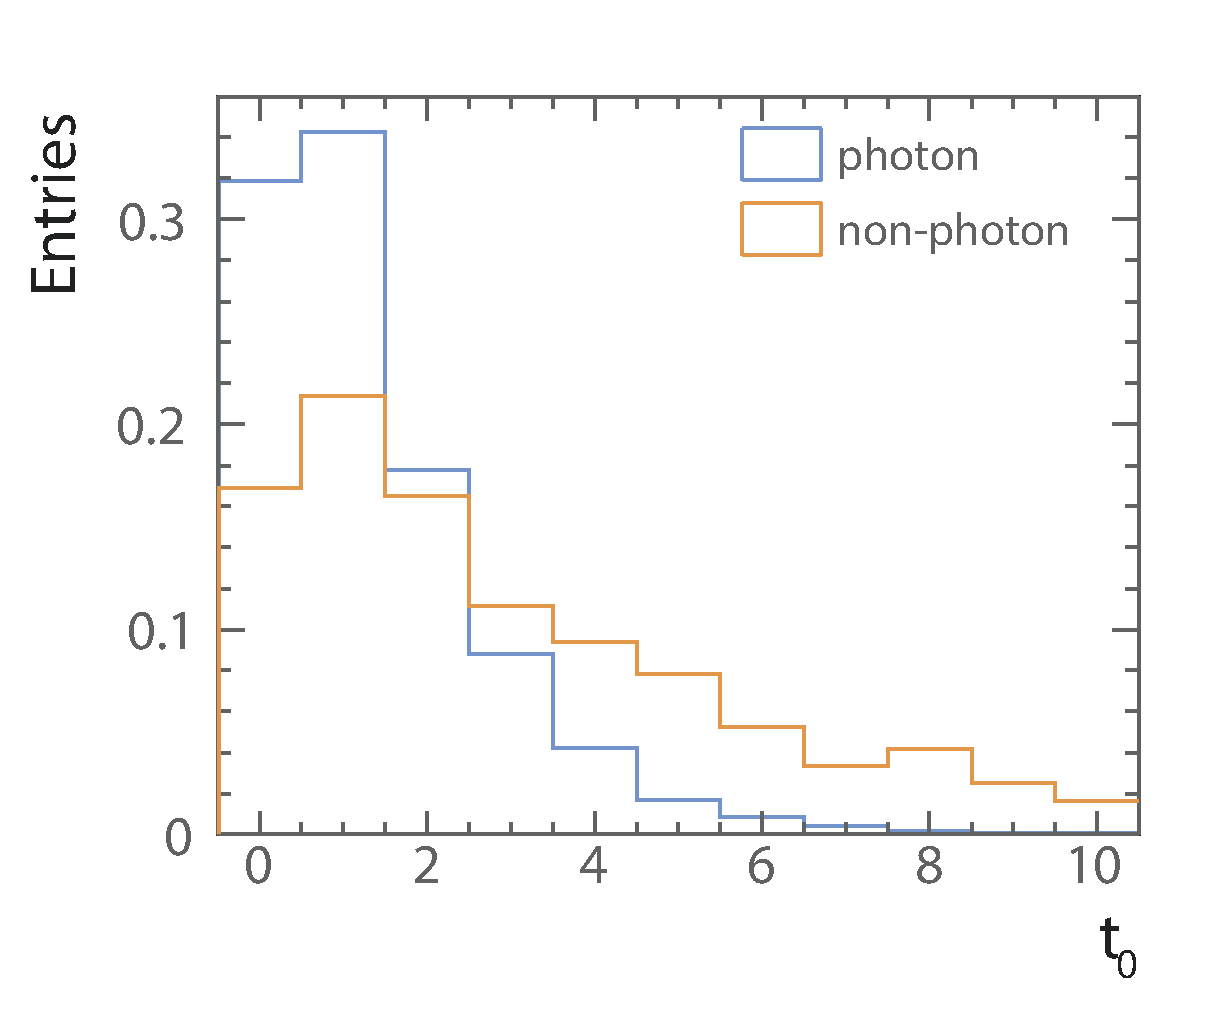
\includegraphics[width=\textwidth]{photon/likelihood/LongProfileStart2}
    \caption{}
    \label{fig:photonLongProfileStart}
  \end{subfigure}
  \begin{subfigure}[b]{0.45\textwidth}
    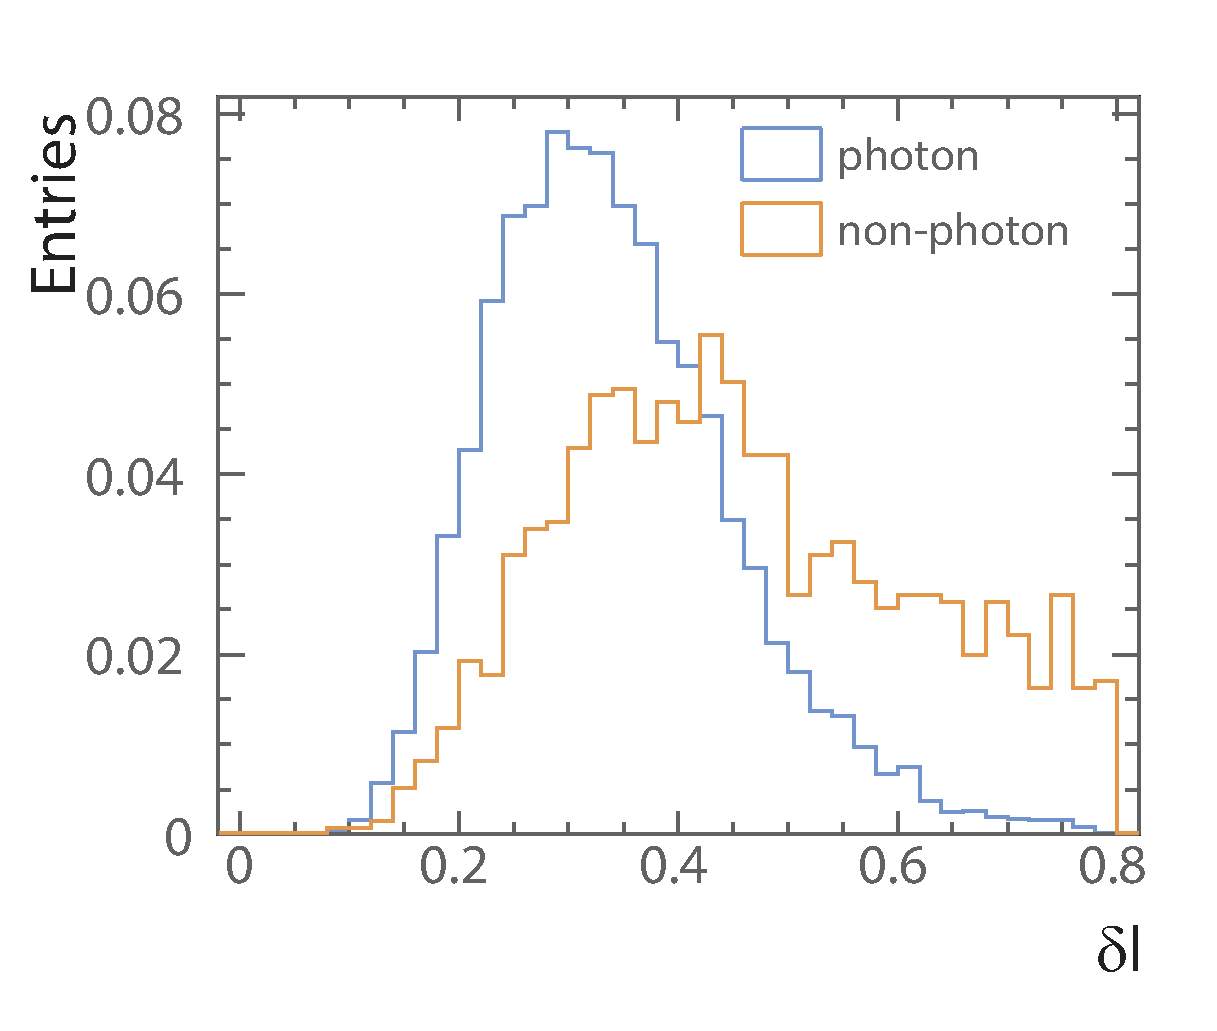
\includegraphics[width=\textwidth]{photon/likelihood/LongProfileDiscrepancy2}
    \caption{}
    \label{fig:photonLongProfileDiscrepancy}
  \end{subfigure}
  \begin{subfigure}[b]{0.45\textwidth}
    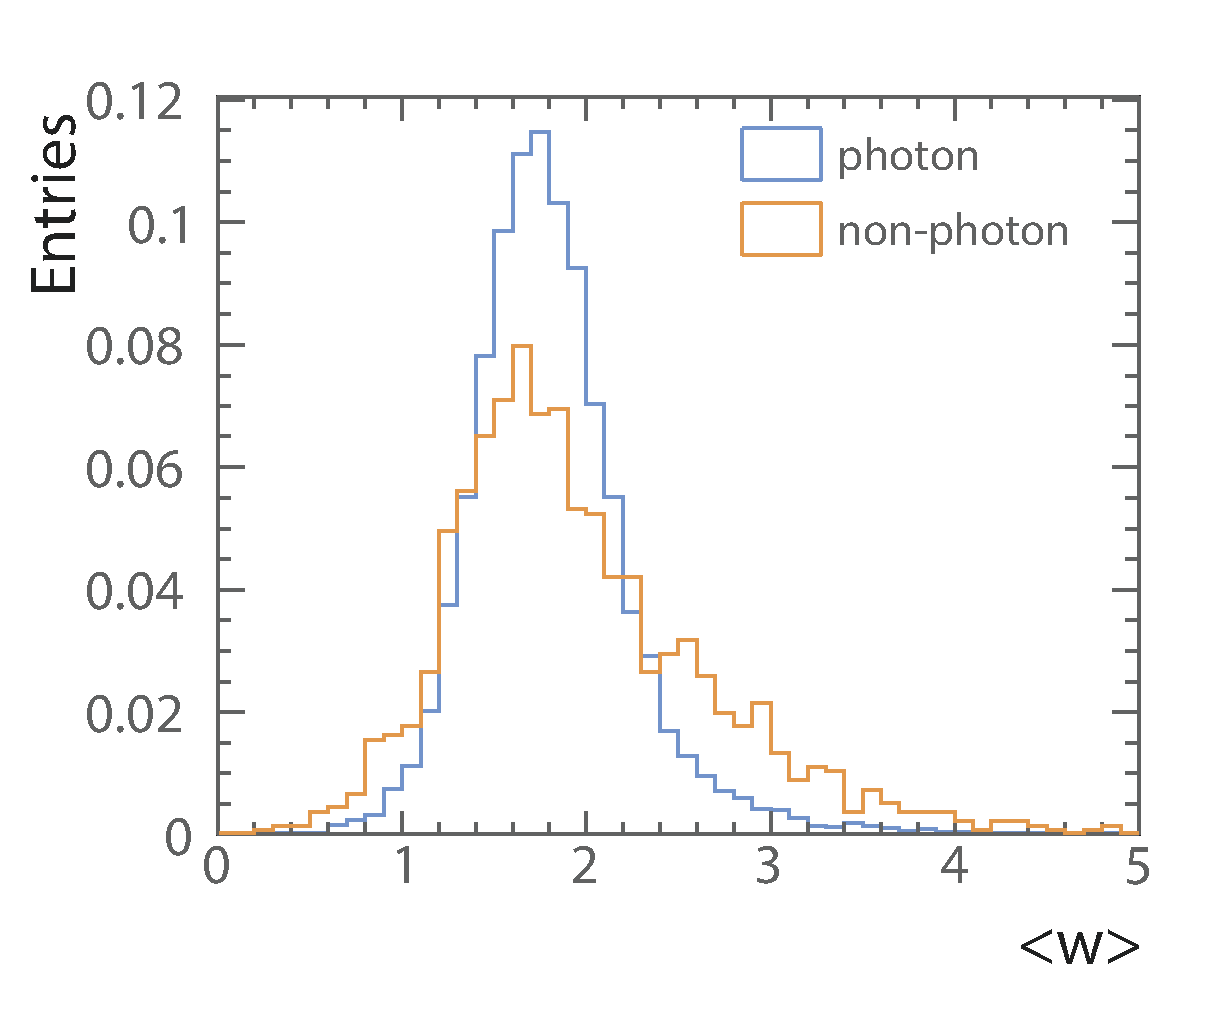
\includegraphics[width=\textwidth]{photon/likelihood/PeakRms2}
    \caption{}
    \label{fig:photonPeakRms}
  \end{subfigure}
  \begin{subfigure}[b]{0.45\textwidth}
    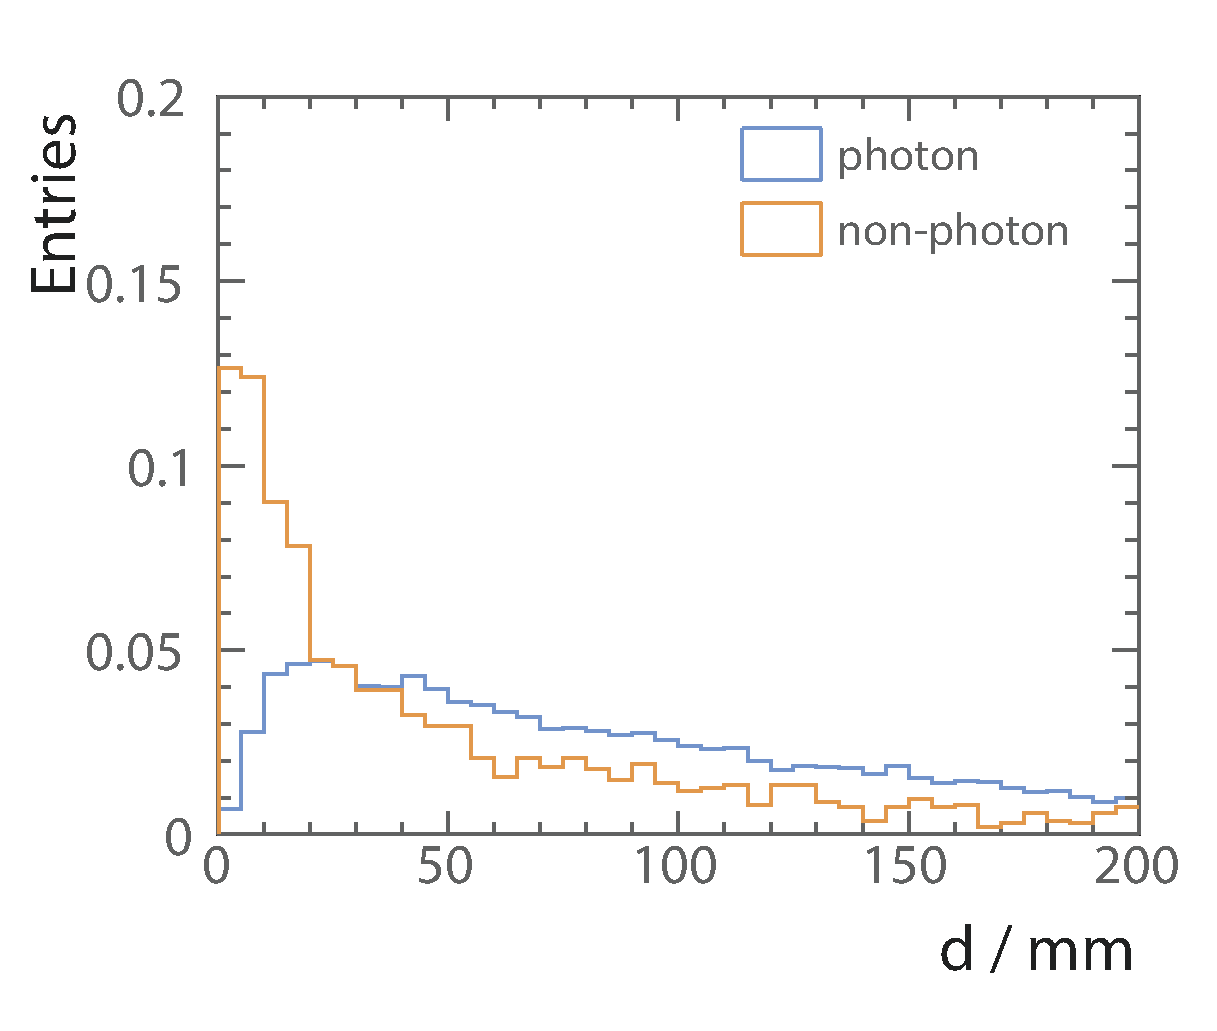
\includegraphics[width=\textwidth]{photon/likelihood/MinDistanceToTrack2}
    \caption{}
    \label{fig:photonMinDistanceToTrack}
  \end{subfigure}
\caption
{Distributions for a) the start layer from the longitudinal shower profile ($t_0$), b)  the fractional difference of the observed shower profile to the expected EM shower profile ($\delta{l}$), c) the energy weighted root-mean-squared distance of all bins in a \ShowerPeak to its peak bin ($\langle{w}\rangle$), and d) the distance between the photon candidate and the closest track projection in the front of the \ECAL ($d$) are shown. All plots are normalised, shown for photons and non-photons, where the particle ID is determined using the truth information. All plots are generated with  simulated 500\,GeV \Zprime events, where  \Zuds.}
\label{fig:photonVarLikelihood}
\end{figure}



%  Candidate with energy below 0.2\,GeV would not be examined in this step, as there are far more non-photons than photons and the classifier makes mor.

\subsection{Projective Likelihood classifier}


Projective likelihood classifier  with probability density estimators is used in \pandora for the photon ID due to its simplicity and the low requirement on computing resources. The details on projective likelihood classifier can be found in \Section{sec:pandoraLikelihood}.

The probability distribution of each variable for photons and non-photons are obtained in the training stage. The distributions of these variables are normalised to probability distribution, stored in binned histograms. The classifier is improved by realising the variable distributions varies with photon energies. Thus the variables distributions are stored separately for different photon energies. There are default 8 energy bins, cutting at 0.2, 0.5, 1, 1.5, 2.5, 5, 10, 20\,GeV, which covers a good range of photon energies. The classifier training typically uses simulated 250\,GeV jet events, with sample \Zuds. High energy jets allow the training for high energy photon candidates.

%Thus these distributions are divided by a range of photon energies. The default energy bins edges are

After training, for a given photon candidate with the energy in the energy bin $\alpha$, the likelihood classifier output is given by
\begin{equation}
pid = \frac{N_p^\alpha \prod_{i}^6{P_{i,p}^\alpha}}{N_p^\alpha\prod_{i}^6{P_{i,p}^\alpha} + N_{np}^\alpha\prod_{i}^6{P_{i,np}^\alpha}}
\end{equation}
where $P^\alpha_{i,p}$ and $P^\alpha_{i,np}$ are the probability of the   $i^{th}$ variable  of the photon candidate fallen in the probability $i^{th}$ variable  distribution of the photon and non-photons in the energy bin $\alpha$, respectively; $N^\alpha_{p}$ and $N^\alpha_{np}$ are the number of the photon and non-photons in the energy bin $\alpha$, respectively.


During classification, a photon candidate passes the photon ID test if
\begin{equation}
\begin{cases}
  pid > 0.6, & \text{if}\ 0.2 < E < 0.5\,GeV\\
  pid > 0.4, & \text{if}\ E \geqslant 0.5\,GeV
\end{cases}
\end{equation}
where $E$ is the photon candidate energy. Two values of the $pid$ cuts reflect the confidence of the photon ID test with different candidate energies. The test is more cautious with low-energy candidates.


\section{Photon fragment removal algorithm in the \ECAL}
\label{sec:photonFragRemoval}
During the reconstruction, it is possible that a core of the photon electromagnetic shower is identified as a photon (the main photon). The outer part of the shower could be reconstructed as a separate particle, and be wrongly identified as a photon or a neural hadron. \FIGURE{fig:photonEvtDspPhotonFrag} shows a typical creation of such a photon fragment. A fragment does not have the electromagnetic shower structure, and typically it has much lower energy than a proper photon. If a photon-fragment pair is merged, the pair should be consistent with an one-particle profile.

\begin{figure}[tbph]
\centering

  \begin{subfigure}[b]{0.3\textwidth}
    
\includegraphics[width=\textwidth]{photon/allPhoton}
    \caption{}
    \label{fig:photonEvtDspPhotonFragAll}
  \end{subfigure}
  \begin{subfigure}[b]{0.3\textwidth}
    
\includegraphics[width=\textwidth]{photon/big}
    \caption{}
    \label{fig:photonEvtDspPhotonFragBig}
  \end{subfigure}
  \begin{subfigure}[b]{0.3\textwidth}
    
\includegraphics[width=\textwidth]{photon/small}
    \caption{}
    \label{fig:photonEvtDspPhotonFragSmall}
  \end{subfigure}

\caption
{An event display of a typical 10\,GeV photon (\Figure{fig:photonEvtDspPhotonFragAll}), reconstructed into a main photon (\Figure{fig:photonEvtDspPhotonFragBig}) and a photon fragment (\Figure{fig:photonEvtDspPhotonFragSmall}). }
\label{fig:photonEvtDspPhotonFrag}
\end{figure}


Photon fragment removal algorithms can exist at difference places in the reconstruction: immediately after the \PhotonReconstruction algorithm (see \SECTION{sec:photonRecoFragRemoval}), or after the charged particle reconstruction. Since these algorithms share the same logics, they will be discussed together. The algorithm used   after the charged particle reconstruction will be discussed here. The algorithm  immediately after the \PhotonReconstruction  differs mostly in the default cut-off values in the  merging metrics.

Spatially close photon and a potential fragment form a pair of particles (photon-fragment pair). Kinematic and topological properties of a photon-fragment pair are examined. The pair is merged when its properties pass a set of cuts, where cuts are developed by comparing true photon-fragment pairs and non photon-fragment pair. This merging test is iterated over all possible  photon-fragment pairs. If multiple photon-fragment pairs with the same photon pass the merging test, the pair with closest distance metric, $d$, will be merged.

The photon-fragment pairs is classified into photon-photon-fragment pairs and photon-neutral-hadron-fragment pairs, because they have different kinematic and topological distributions. The pairs are further classified into low energy and high energy pairs, depending on whether the fragment energy ($E_p$) is above 1\,GeV. The cuts for merging pairs are listed in \Table{tab:photonFragRemovalCuts}.



\TABLE{tab:photonFragRemovalCuts} lists cuts for merging photon-photon-fragment pairs and photon-neutral-hadron-fragment pairs for both low energy and high energy fragments. $d$, $d_c$ and $d_h$ are mean energy weighted intra-layer distance within the pair, distance between two centroids, and minimum distance between calorimeter hits of each \PFO in the pair, respectively.  Three distance measurements have subtle difference. $d_c$ gives the distance between centroids of each \PFO in the pair, which is a computationally quick but crude measurement. $d_h$ is the minimum distance between calorimeter hits of each \PFO in the pair. For a true photon-fragment, $d_h$ should be close to zero as the pair should be spatially close. $d$ is the mean energy weighted intra-layer distance between  each \PFO in the pair (see \Figure{fig:photonDistanceMetric}):
\begin{equation}
d = \frac{\sum_{i}^{layers}d_{l,i}\ E_{f,i}}{\sum_{i}^{layers}E_{f,i}}
\end{equation}
where $i$ indicates $i^{th}$ pseudo-layer of the \ECAL. $d_{l,i}$ is the minimum distance between calorimeter hits of the pair in the $i^{th}$ pseudo-layer. $E_{f,i}$ is the energy of the fragment in the $i^{th}$ pseudo-layer. $d$ is a better measurement of the closeness of the pair. All three distance metrics should be small to merge a photon-fragment pair.

\begin{figure}[tbph]
\centering
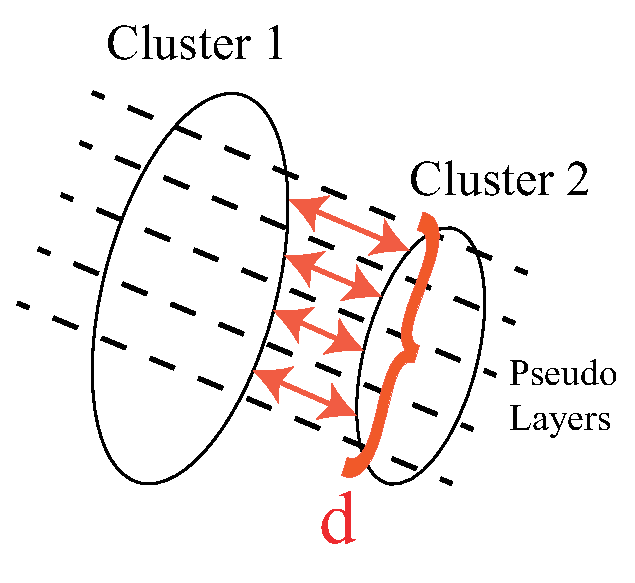
\includegraphics[width=0.45\textwidth]{photon/dLayer}
\caption{Illustration of distance metric, $d$.}
\label{fig:photonDistanceMetric}
\end{figure}

$E_m$ and $E_f$ are the main photon energy and the fragment energy. $E_{p1}$ and $E_{p2}$ are the two largest peaks and associated calorimeter hits, found by the \peakFinding algorithm (\Section{sec:peakFinding}), ordered by descending energy, using the pair as input. $N_{calo}$ is the number of the \ECAL hits in the fragment. $\absCosTheta$ is the absolute cosine of the polar angle of the main photon, where beam direction is the z-axis.

One logic for merging is when the fragment has low energy and is close to the main photon. Hence $E_f$  and $N_{calo}$ are required to be small. Alternatively the fragment should be relatively low energetic, demanding a small ratio of $E_f$ to $E_m$.

The other logic is when the pair looks like one photon in two-dimensional energy deposition projection (see \Section{sec:photonCandiate} and \Figure{fig:photonPeakFinding}). The transverse shower comparison requires $\frac{E_{p1}}{E_m + E_f} > 0.9 $, where most energy contains in the first \ShowerPeak object.

Comparing cuts with low $E_f$ and high $E_f$, the cuts are similar. Cuts for high $E_f$ allow higher energy fragments to be merged.

Comparing photon-photon-fragment pair and photon-neutral-hadron-pair, cuts for photon-neutral-hadron-pair are more conservative for low $E_f$, but more relaxed for high $E_f$. This reflects that the neutral hadron fragments originated from charged particles are more likely to be low energy, whilst high energy neutral fragments are more likely to be photon fragments.

Since all possible photon-fragment pairs are compared, this is a costly cooperation with $O(n^2)$ time complexity for $n$ particles. The speed is improved by considering only the pairs with $d<80\ \text{mm}$.

\begin{table}[htbp]
\centering

\smallskip

\begin{tabular}{l  r  r }
\hline
\hline
Low $E_f$ &  Photon-photon & Photon-neutral-hadron \\
\hline
\multicolumn{1}{L{0.3\textwidth}}{transverse shower comparison} & \multicolumn{1}{R{0.3\textwidth}}{$d < 30 $, $\frac{E_{p1}}{E_m + E_f} > 0.9 $, $\frac{E_{p2}}{E_f} < 0.5 $, $E_{p1} > E_m$}  & \multicolumn{1}{R{0.3\textwidth}}{-} \\
\multicolumn{1}{L{0.3\textwidth}}{close proximity} & \multicolumn{1}{R{0.3\textwidth}}{-}  & \multicolumn{1}{R{0.3\textwidth}}{$d < 20 $, $d_c < 40 $} \\
\multicolumn{1}{L{0.3\textwidth}}{low energy fragment} & \multicolumn{1}{R{0.3\textwidth}}{$d < 20 $, $E_p < 0.4 $}  & \multicolumn{1}{R{0.3\textwidth}}{-} \\
\multicolumn{1}{L{0.3\textwidth}}{small fragment 1} & \multicolumn{1}{R{0.3\textwidth}}{$d < 30 $, $N_{calo} < 40 $, $d_c < 50 $}  & \multicolumn{1}{R{0.3\textwidth}}{$d < 50 $, $N_{calo} < 10 $, $d_h < 50$} \\
\multicolumn{1}{L{0.3\textwidth}}{small fragment 2} & \multicolumn{1}{R{0.3\textwidth}}{$d < 50 $, $N_{calo} < 20 $}  & \multicolumn{1}{R{0.3\textwidth}}{-} \\
\multicolumn{1}{L{0.3\textwidth}}{small fragment forward region} & \multicolumn{1}{R{0.3\textwidth}}{$N_{calo} < 40$, $d_c < 60$, $E_f < 0.6$, $\absCosTheta > 0.7$}  & \multicolumn{1}{R{0.3\textwidth}}{-} \\
\multicolumn{1}{L{0.3\textwidth}}{relative low energy fragment} & \multicolumn{1}{R{0.3\textwidth}}{$d < 40$, $d_h < 20$, $\frac{E_{f}}{E_m} < 0.01$}  & \multicolumn{1}{R{0.3\textwidth}}{$d < 40$, $d_h < 15$, $\frac{E_{f}}{E_m} < 0.01$} \\
\hline
High $E_f$ &  Photon-photon & Photon-neutral-hadron \\
\hline
\multicolumn{1}{L{0.3\textwidth}}{transverse shower comparison} & \multicolumn{1}{R{0.3\textwidth}}{$\frac{E_{p1}}{E_m + E_f} > 0.9 $, $E_{p2} = 0$ or ($\frac{E_{p2}}{E_f} < 0.5 $, $E_{p1} > E_m$)}  & \multicolumn{1}{R{0.3\textwidth}}{$\frac{E_{p1}}{E_m + E_f} > 0.9 $, $E_{p2} = 0$ or ($\frac{E_{p2}}{E_f} < 0.5 $, $E_{p1} > E_m$)} \\
\multicolumn{1}{L{0.3\textwidth}}{relative low energy fragment 1} & \multicolumn{1}{R{0.3\textwidth}}{$d < 40$, $d_h < 20$, $\frac{E_f}{E_m} < 0.02$} & \multicolumn{1}{R{0.3\textwidth}}{$d < 40$, $d_h < 20$, $\frac{E_f}{E_m} < 0.02$} \\
\multicolumn{1}{L{0.3\textwidth}}{relative low energy fragment 2} & \multicolumn{1}{R{0.3\textwidth}}{-}  & \multicolumn{1}{R{0.3\textwidth}}{$d < 40$, $d_h < 20$, $\frac{E_f}{E_m} < 0.1$, $E_f > 10$} \\
\multicolumn{1}{L{0.3\textwidth}}{relative low energy fragment 3} & \multicolumn{1}{R{0.3\textwidth}}{-}  & \multicolumn{1}{R{0.3\textwidth}}{$d < 20$, $d_h < 20$, $\frac{E_f}{E_m} < 0.2$, $E_f > 10$} \\
\hline

\hline
\end{tabular}

\caption[The cuts for photon fragment removal algorithm in the \ECAL.]%
{The cuts for merging photon-photon-fragment pairs and photon-neutral-hadron-fragment pairs for both low energy and high energy fragments. $d$, $d_c$ and $d_h$ are the mean energy weighted intra-layer distance of the pair, the distance between centroids, the minimum distance between calorimeter hits of the pair. $E_m$ and $E_f$ are the main photon energy and the fragment energy. $E_{p1}$ and $E_{p2}$ are the two largest peaks, found by peak finding algorithm, ordered by descending energy. $N_{calo}$ is the number of the calorimeter hits in the fragment. $\absCosTheta$ is the absolute cosine of the polar angle, where beam direction is the z-axis.}
\label{tab:photonFragRemovalCuts}
\end{table}


\section{Photon fragment recovery algorithm in the \HCAL}
\label{sec:photonHighEFragRemoval}

\SECTION{sec:photonFragRemoval} descried an effective algorithm to removal photon fragments that are peripheral to the main photon, the electromagnetic shower core. There is another type of fragments originated from the leakage effect of the \ECAL. An example of a 500\,GeV photon reconstructed into a main photon in the \ECAL (yellow) and a neutral hadron fragment in the \HCAL (blue) is shown in \Figure{fig:photonEvtDspHCalFrag}.  When a high energy EM shower is not fully contained in the \ECAL, shower deposits energy in the \HCAL, which often forms a neutral hadron in the \HCAL. Previous algorithms only consider calorimeter hits in the \ECAL.  Therefore no attempts have been made to recover photon fragments in the \HCAL. This section presents an algorithm to merge photon fragments in the \HCAL. This photon fragment recovery algorithm is important when reconstructing  high energy photons. For the \ILD detector, this \ECAL leakage effect appears when the photon energy is above 50\,GeV.


\begin{figure}[tbph]
\centering
{
\includegraphics[width=0.5\textwidth]{photon/hcalfrag}}%
\caption{An event display of a typical 500\,GeV photon, reconstructed into a main photon in the \ECAL (yellow) and a neutral hadron fragment in the \HCAL (blue).}
\label{fig:photonEvtDspHCalFrag}
\end{figure}

Shown in  \Figure{fig:photonEvtDspHCalFrag}, photon fragments in the \HCAL is  spatially close to the main photon. A fitted cone from the main photon, if extended to the \HCAL, covers most of the fragment. These features allow a set of cuts developed to merge  fragments in the \HCAL, listed in \Table{tab:photonHighEnergyFragCuts}.

This algorithm would collect photons in the \ECAL and neutral hadrons in the \HCAL as inputs. The algorithm then iterates over all pairs of reconstructed photons and neutral hadrons. For each pair, a set of variables are calculated and compared to a set of cuts (\Table{tab:photonHighEnergyFragCuts}). Photon-fragment pairs passing the cuts will be merged.


Fragment in the \HCAL should be spatially close to the main photon, measured by three metrics. $d^l_c$ is the distance between centroids of the last outer layer of the main photon and the first inner layer of the fragment. $d^l_{fit}$ is the distance between fitted directions using the last outer layer of the main photon and the first inner layer of the fragment. $d_{fit}$ is the distance between fitted directions using the main photon and the fragment. These three distances should be small for merging.

The direction of the fragment should be similar to the direction of the main photon. $r_f$, the root-mean-square energy weighted distance of a calorimeter hit in the fragment to the direction of the main photon, has to be small for merging.

Another feature of the fragment and the main photon is that the shower width should be similar. $w^l_m$ and $w^l_f$ are the r.m.s. width of the last outer layer of the main photon and the first inner layer of the fragment. The ratio $\frac{w^l_f}{w^l_m}$ needs to be in the range of 0.3 to 5. The generous upper bound is because the \HCAL cell size is much larger than that of the cell size of the \ECAL.

When a fitted cone from the main photon is extended to the \HCAL, the cone should contain a significant amount of the fragment. $\%{N}$, the fraction of the calorimeter hits in the fragment in the extended fitted cone of the main photon, has to be no less than 0.5 for the merging.

The last criteria is the fragment should has low energy relative to the main photon. $E_m$ and $E_f$ are the main photon energy and the fragment energy. The ratio, $\frac{E_f}{E_m}$, has to be less than 0.1 for the merging.

If multiple photon-fragment pairs pass the cuts with the same fragment, the pair with highest $\%{N}$ will be merged.

This \HCAL fragment removal algorithm occurs after the first pass of topological association in the reconstruction which connects tracks to clusters in the calorimeters.



\begin{table}[htbp]
\centering

\smallskip

\begin{tabular}{l r }
\hline
\hline
High energy fragment recovery&  Cuts\\
\hline
\multicolumn{1}{L{0.3\textwidth}}{distance comparison} & \multicolumn{1}{R{0.3\textwidth}}{$d^l_c \leqslant 173\ \text{mm}$, $d^l_{fit} \leqslant 100\ \text{mm}$, $d_{fit} \leqslant 100\ \text{mm}$} \\
\multicolumn{1}{L{0.3\textwidth}}{shower width comparison} & \multicolumn{1}{R{0.3\textwidth}}{$  0.3 \leqslant \frac{w^l_f}{w^l_m} \leqslant 5$} \\
\multicolumn{1}{L{0.3\textwidth}}{projection comparison} & \multicolumn{1}{R{0.3\textwidth}}{$ r_f \leqslant 45\ \text{mm}$} \\
\multicolumn{1}{L{0.3\textwidth}}{energy comparison} & \multicolumn{1}{R{0.3\textwidth}}{$ \frac{E_f}{E_m} \leqslant 0.1$} \\
\multicolumn{1}{L{0.3\textwidth}}{cone comparison} & \multicolumn{1}{R{0.3\textwidth}}{$ \%{N} \geqslant 0.5$} \\
\hline

\hline
\end{tabular}

\caption[Cuts for merging high energy photon fragment in the \HCAL.]%
{The cuts for merging high energy photon fragment in the \HCAL to the main photon in the \ECAL. $d^l_c$ is the distance between centroids of the last outer layer of the main photon and the first inner layer of the fragment. $d^l_{fit}$ is the distance between fitted directions using the last outer layer of the main photon and the first inner layer of the fragment. $d_{fit}$ is the distance between fitted directions using the main photon and the fragment. $w^l_m$ and $w^l_f$ are the  root-mean-squared width of the last outer layer of the main photon and the first inner layer of the fragment. $r_f$ is the root-mean-squared energy weighted distance of a calorimeter hit in the fragment to the direction of the main photon. $E_m$ and $E_f$ are the main photon energy and the fragment energy. $\%{N_{calo,cone}}$ is the fraction of the calorimeter hits in the fragment in the extended fitted cone of the main photon.}
\label{tab:photonHighEnergyFragCuts}
\end{table}

\section{Photon splitting algorithm}
\label{sec:photonSplitting}

Algorithms described above deal with forming photons from calorimeter hits in the \ECAL, merging photon fragments in the \ECAL and the \HCAL. Another aspect in photon reconstruction is splitting accidentally merged photons. During the particle reconstruction, it is possible that photons are accidentally merged if they are spatially close. Hence another algorithm at the end of the particle reconstruction addresses this issue and tries to split merged photons. This algorithm focuses on energetic photons with energy > 10\,GeV.

%Merged photons are typically energetic.
A merged photon should be consistent with topologies of a spatially closed photon pair. Extra care should be taken if the photon is close to a charged tracks. Many \pandora algorithms deal with track clusters association and there is a great confidence in clusters associated with tracks.


\TABLE{tab:photonPhotonSplitting} lists the cuts used in the algorithm. $E$ is the photon energy. $E_{p2}$ is  energy of the second largest peak from the \peakFinding algorithm. If an energetic photon (cut on $E$) is identified, and two energetic EM showers (cut on $E_{p2}$) can be found at the same time, the photon should be split according to the \peakFinding results.

When the candidate is close to a charged track, which is defined as within 100\,mm of the track projection on the front of the \ECAL, extra care is taken by demanding a large value for second EM shower energy. $E_{c1}$ and $E_{c2}$ are the energy cut-off values, determined by the number of nearby charged track.

The restraint on $N_{p}$, the number of peaks identified by the peak finding, is needed because one reconstructed photon is unlikely to be merged from more than four photons.


\begin{table}[htbp]
\centering
\smallskip
\begin{tabular}{l r }
\hline
\hline
Photon splitting&  Cuts\\
\hline
\multicolumn{1}{L{0.3\textwidth}}{Cuts} & \multicolumn{1}{R{0.3\textwidth}}{$E > E_{c1}$, $E_{p2} > E_{c2}$, $N_{p} < 5$} \\
\hline
$E_{c1}$ and $E_{c2}$ values &  \\
\hline
\multicolumn{1}{L{0.3\textwidth}}{0 charged \PFO nearby} & \multicolumn{1}{R{0.3\textwidth}}{$E_{c1} = 10$, $E_{c2} = 1$} \\
\multicolumn{1}{L{0.3\textwidth}}{1 charged \PFO nearby} & \multicolumn{1}{R{0.3\textwidth}}{$E_{c1} = 10$, $E_{c2} = 5$} \\
\multicolumn{1}{L{0.3\textwidth}}{> 1 charged \PFO nearby} & \multicolumn{1}{R{0.3\textwidth}}{$E_{c1} = 20$, $E_{c2} = 10$} \\
\hline

\hline
\end{tabular}

\caption[Cuts for splitting photons.]%
{The cuts for splitting photons, and the values for energy cut-off points. $E$ is the photon energy. $E_{p2}$ is  energy if the second largest peak from the two dimensional peak finding. $N_{p}$ is the number of peaks identified by the peak finding. $E_{c1}$ and $E_{c2}$ are the energy cut-off values, determined by the number of nearby charged \PFO{s}.}
\label{tab:photonPhotonSplitting}
\end{table}

\section{Characterise the performance}


Motivations and implementations of four different photon related algorithms have been described above. The main photon reconstruction algorithm in \Section{sec:photonRecostrcution} improves the photon completeness and the photon pair resolution, due to the improved two dimensional peak finding algorithm in \Section{sec:peakFinding}. The fragment removal algorithms in \Section{sec:photonFragRemoval} and \Section{sec:photonHighEFragRemoval} further reduce the photon fragments in the \ECAL and the \HCAL. The photon splitting algorithm in \Section{sec:photonSplitting} exploits the peak finding algorithms to separate photons using transverse shower information, which improves the photon separation resolution. Photon reconstruction improves single photon resolutions. It also improves jet energy resolution at high \sqrtS because of the high photon reconstruction completeness.

Three different versions of the \pandora are used to characterise  the performance.
\begin{itemize}
  \item No stand-alone photon reconstruction algorithms
  \item With a stand-alone photon reconstruction algorithm from \pandora version 1.
  \item With full photon related algorithms described above, incorporated in \pandora version 3.
\end{itemize}

First the performance with the full algorithms is compared with no photon algorithms, then compared with \pandora version 1. The individual photon related algorithms are then characterised, followed by performance of the photon reconstruction in \pandora version 3.

\section{Compare with no photon reconstruction}

This section compares the performance with and without photon related algorithms using photon pair and jet samples. The nominal \ILD detector model is used. The single photon events were generated with an uniform distribution in the solid angle of the photon. The two photon events were generated with an uniform distribution in the solid angle of the first photon, and an uniform distribution in the solid angle  for a range of the opening angles between the pair. Events are selected such that there is no early photon conversion in the tracking detector and the photon deposits energies in the calorimeter. The events are further restricted to photon decaying in barrel and end cap region only, to minimise the detector effect.


\FIGURE{fig:photonDoublePerformanceNoReco} shows the photon reconstruction for two spatially close photons  reconstructed without and with photon algorithms. Without the photon related algorithms, fragments are produced.  The number of photons between 0 and 10\,mm separation is around 1.5. The true photon number for that region should be 1, as it is extremely challenging to separate photons less than two cells apart.  Without the photon related algorithms, photon separation resolution is much worse, as the number of photon appears to be flat between 0 to 30\,mm separation. With the photon related algorithms, two photons start to be separated at 10\,mm and fully separated at 20\,mm separation.


\begin{figure}[tbph]
\centering
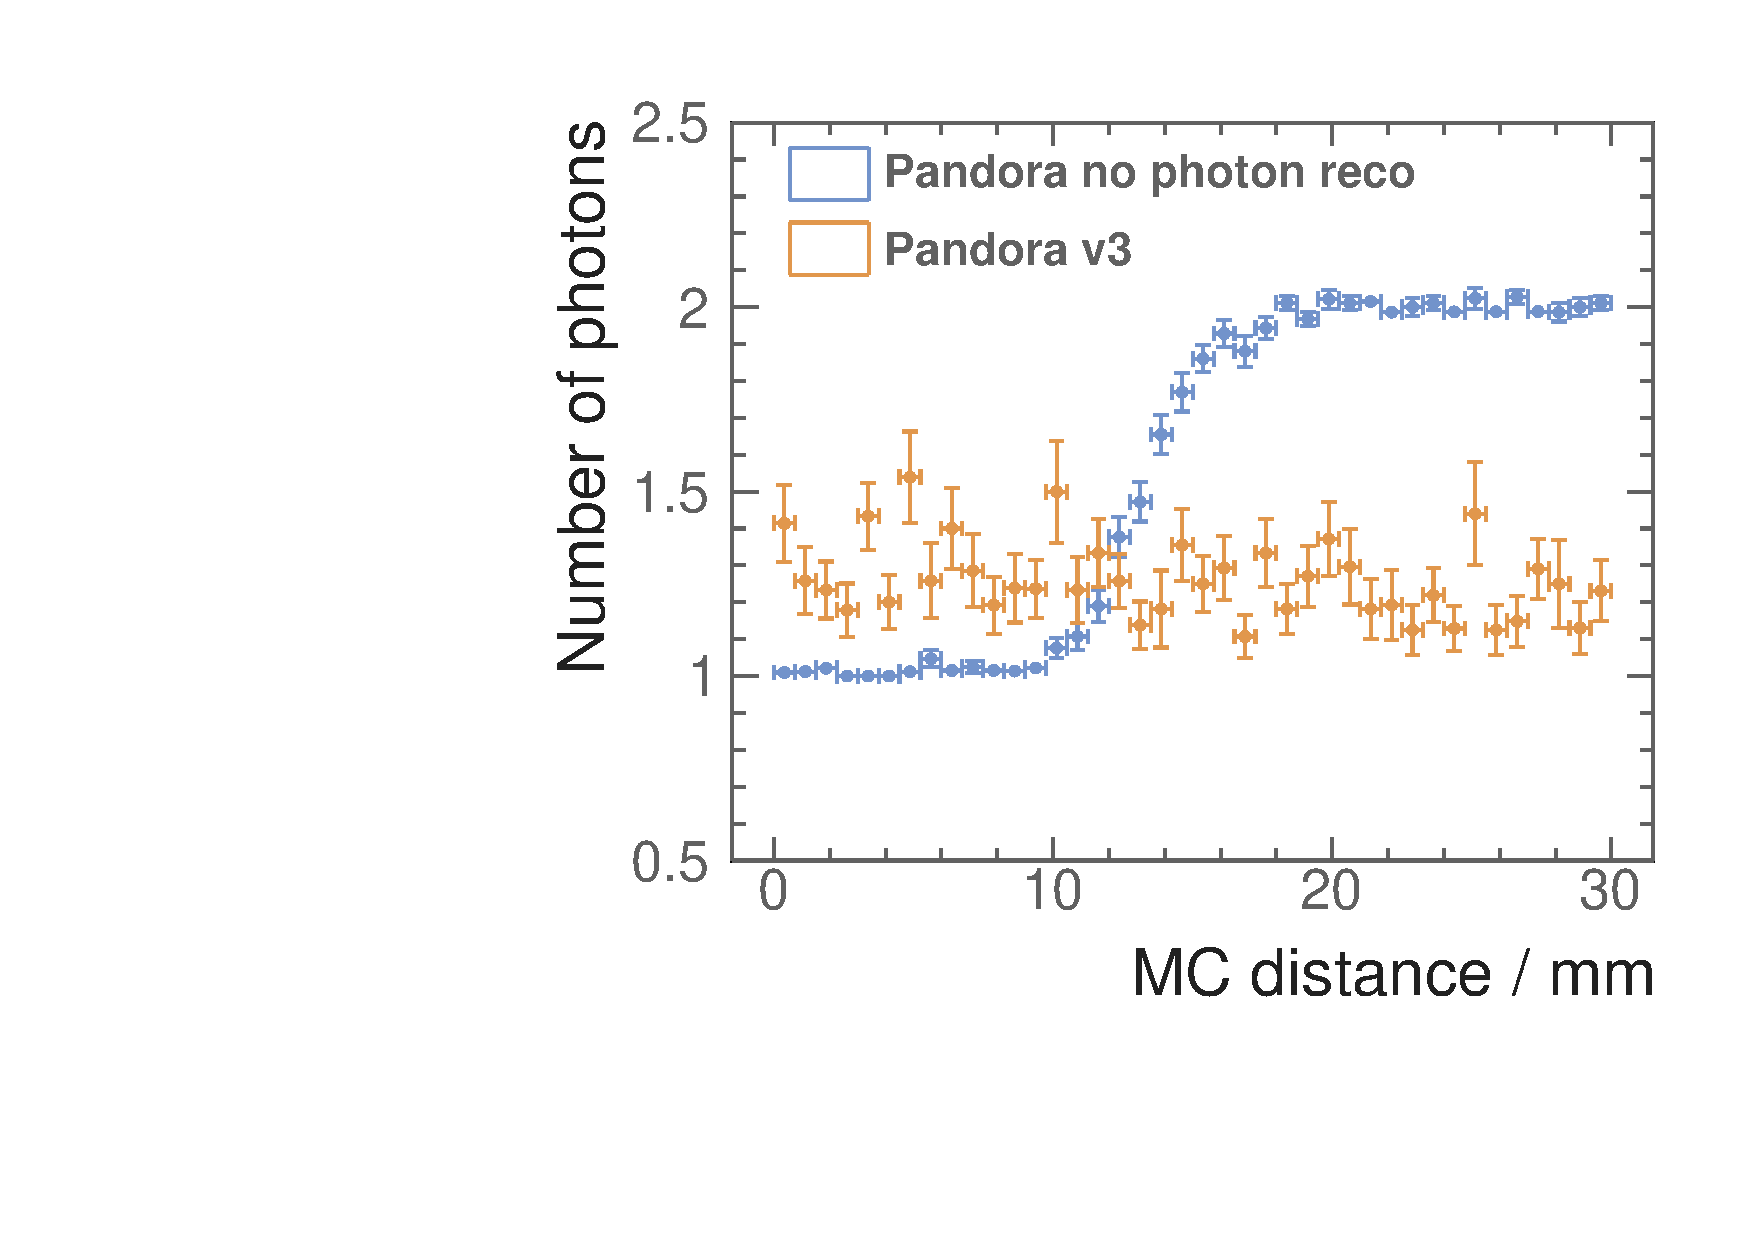
\includegraphics[width=0.45\textwidth]{photon/nPhotonVSnoPhotonReco.pdf}
\caption[Average number of photons using two photons of 500 and 50\,GeV per event sample.]
{Average number of photons using two photons of 500 and 50\,GeV per event sample reconstructed  without and with photon algorithms.}
\label{fig:photonDoublePerformanceNoReco}
\end{figure}




The improvement in completeness and resolution in photon reconstruction, leads to a considerable improvement in the jet energy resolution at high energy. Jet energy resolution is defined as the root mean squared divided by the mean for the smallest width of distribution that contains 90\% of entries, using \Zuds sample at barrel region. The angular cut is to avoid the barrel/endcap overlap region. The light quark decay of the \Zprime is used as \pandora does not attempt to recover missing momentum from semi-leptonic decay of heavy quarks. Using 90\% of the entries is robust and focus on the Gaussian part of the distribution. The total jet energy is sampled at 91, 200, 360 and 500\,GeV. Shown in \Figure{fig:photonJERmuon}, the jet energy resolutions are much better at 360 and 500\,GeV with improved photon reconstruction. By identifying photons before reconstructing charged particles in a dense jet environment, the reconstruction task is easier and less likely to make mistakes. However, at low energy, the reconstruction is worse with photon algorithms, because photon algorithms are optimised for high energies.

\begin{figure}[tbph]
\centering
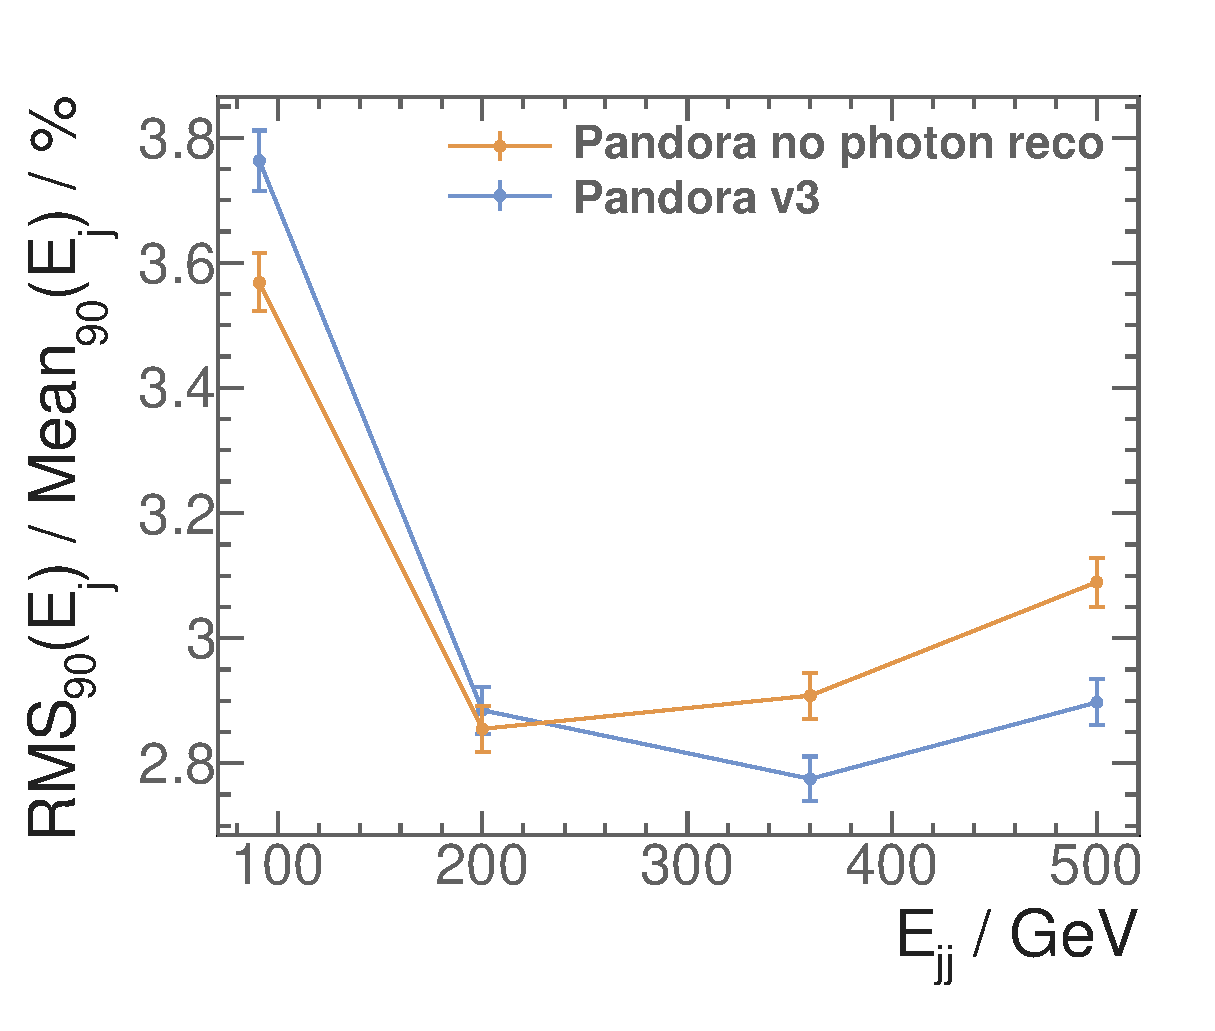
\includegraphics[width=0.45\textwidth]{photon/JERmuon.eps}
\caption[Jet energy resolution as a function of the total jet energy without and with photon related algorithms]
{Jet energy resolution as a function of the  total jet energy using \Zuds sample at barrel region. The top orange and bottom blue dots are reconstructed without and with photon related algorithms.}
\label{fig:photonJERmuon}
\end{figure}


To access the impact of photon algorithms on jet energy resolution, perfect photon reconstruction is used to compare the performances, which identifies calorimeter hits from truth information. Same jet samples are used. Photon confusion, which is defined as the quadrature difference between a normal reconstruction and a perfect photon confusion, is listed in \Table{tab:photonPhotonConfusion}. Photon confusion term, except for \rootSGeV{91}, has been reduced to 0.9\% with the photon algorithms.


\begin{table}[htbp]
\centering
\begin{tabular}{ l   r  r  r  r   }
\hline
\hline
Photon confusion &\rootSGeV{91} & 200\,GeV & 360\,GeV & 500\,GeV  \\
\hline
\multicolumn{1}{L{0.3\textwidth}}{\pandora without photon algorithms}& 0.7\% & 0.9\% & 1.3\% & 1.4\%  \\
\multicolumn{1}{L{0.3\textwidth}}{\pandora with photon algorithms} & 1.4\% & 0.9\% & 0.9\% & 0.9\%  \\
\hline
\hline
\end{tabular}

\caption[Photon confusion as a function of energy for reconstruction with and without photon algorithms.]
{Photon confusion as a function of total jet energy in the \Zuds samples for reconstruction with and without photon algorithms.}
\label{tab:photonPhotonConfusion}
\end{table}

\begin{comment}
    Double_t y2[nPoints] = {3.56892,2.85493,2.90771,3.08924};// MUON /r02/lc/xu/MarlinPandoraTest/HEAD20151210/20151211am10/
    Double_t erry2[nPoints] = {0.0460938,0.036756,0.0370356,0.0396873 };// MUON with 20150413 20150929am14

    //Double_t y2[nPoints] = {3.49641, 2.72426, 2.61667, 2.7686};// perfect photon from steve
    //Double_t erry2[nPoints] = {0.0444942,0.036756,0.0334291,0.0353562 };//


    Double_t y1[nPoints] = {3.76354,2.8844,2.77463,2.89704};// new photon with merging 20160107am13
    Double_t erry1[nPoints] = {0.0482638,0.0371727,0.0357569 ,0.03669   };//
\end{comment}

\section{Compare with photon reconstruction in \pandora version 1}
\label{sec:photonPerformanceCompare}

This section reviews the performance improvement with the introduced algorithms, using single photon, photon pair and jet samples. There is a old photon reconstruction algorithm in \pandora version 1. Since the changes to the photon reconstruction is made in \pandora version 2, \pandora version 3 contains all the algorithms for the photon reconstruction. This section concentrates on the improvement from version 1 to version 3.

%The \ECAL square cell size is about 5\,mm.

%We will review performance metrics of above algorithms. \Fig{fig:n_p} shows the number of reconstructed photons as a function of their true distance separation for a two photons per event sample. The reduction of the number of reconstructed photons are mainly due the the fragment merging algorithms for fragments in the ECal. \Fig{fig:n_all} shows a similar reduction in the reconstructed particles as in \Fig{fig:n_p}, and it shows that neutral hadron fragments in HCal have been merged back to main photons.


Testing samples are generated in the same way as in the previous section. \FIGURE{fig:photonSingleN_p} shows the reduction in fragments identified as photons, using a single photon per event sample. Indicating as the blue dots on the plots, average number of photon stays below 1.05 even at 500 \,GeV (true value 1). For a 100\,GeV photon, the average number of photons is reduced to 1 from 2. For a 500\,GeV photon, the  number is reduced to 1.05 from 2.8.

\begin{figure}[tbph]
\centering
    \begin{subfigure}[b]{0.45\textwidth}
        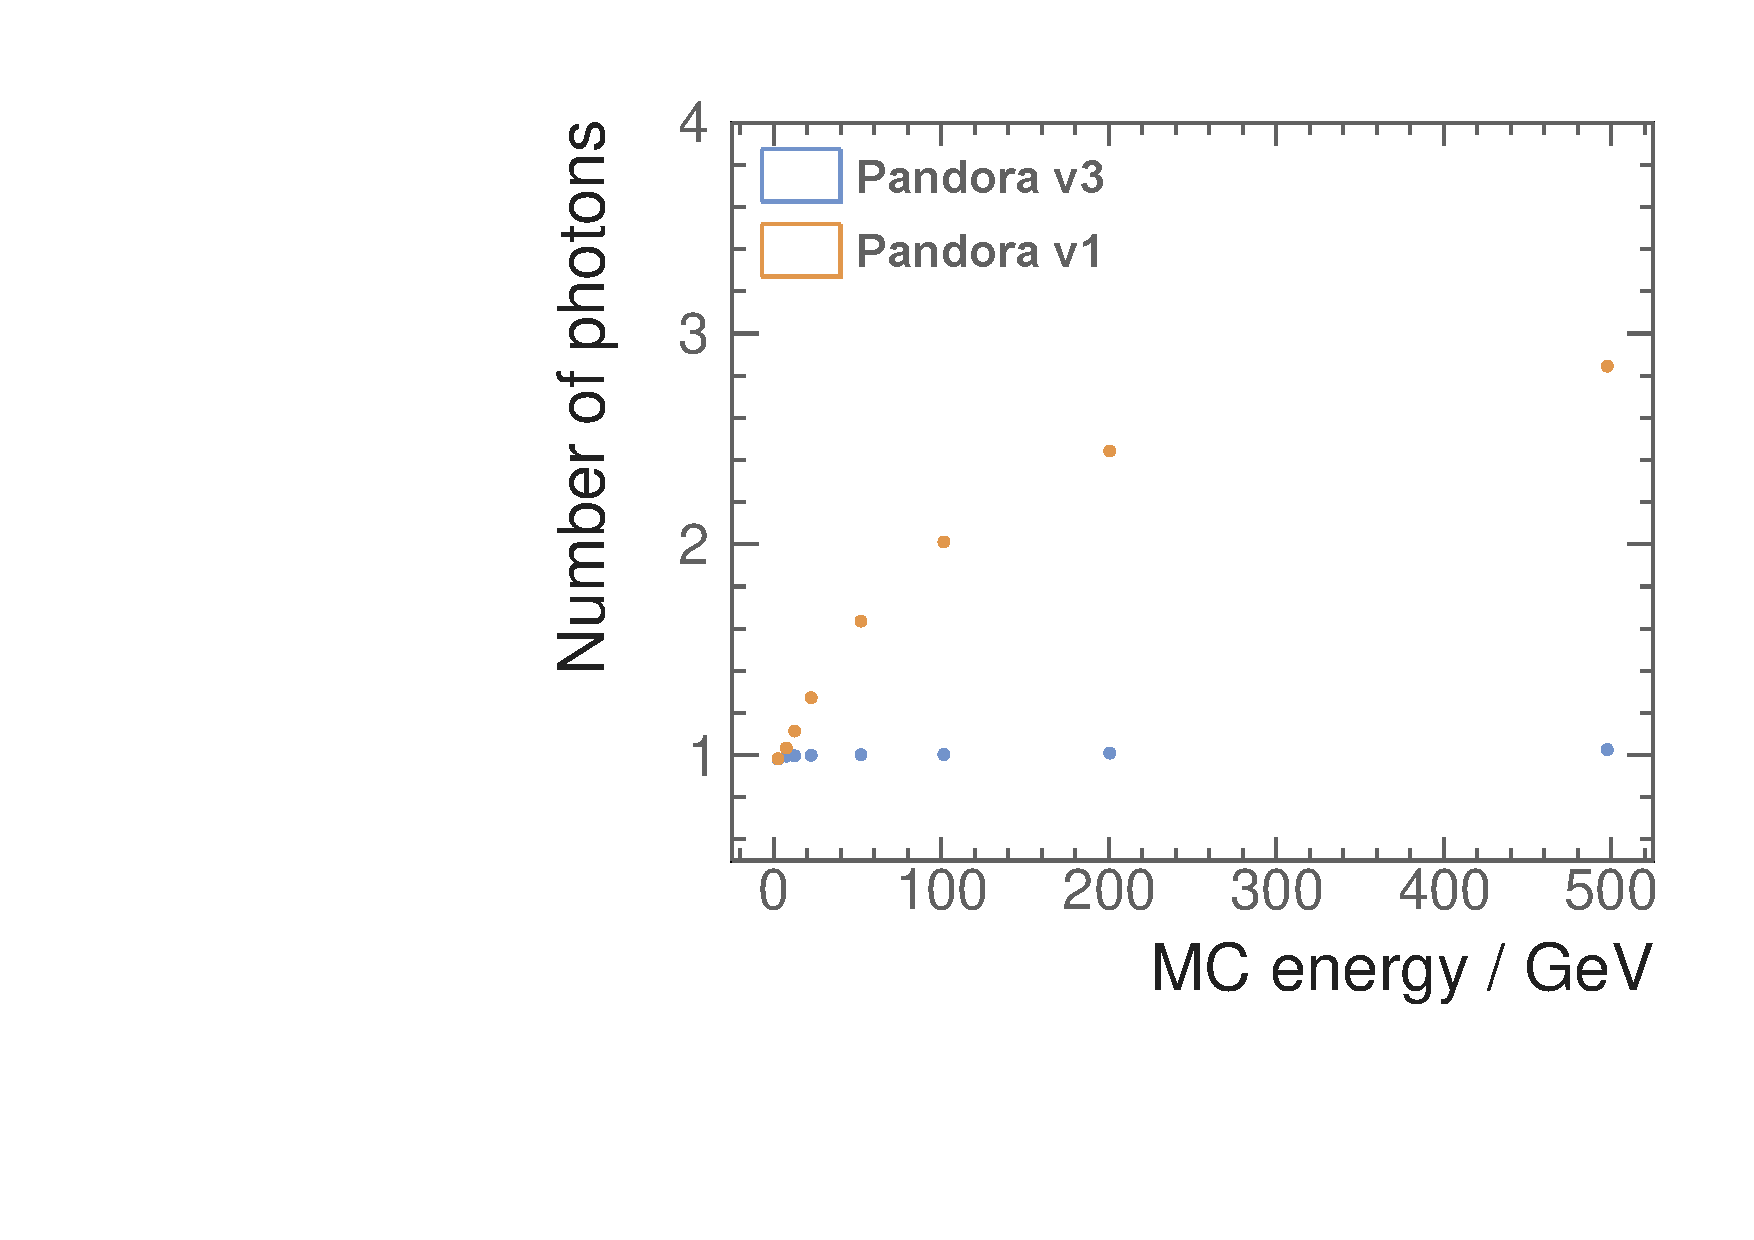
\includegraphics[width=\textwidth]{photon/SingleN_pedit.pdf}
        \caption{}
        \label{fig:photonSingleN_p}
    \end{subfigure}
    \begin{subfigure}[b]{0.45\textwidth}
        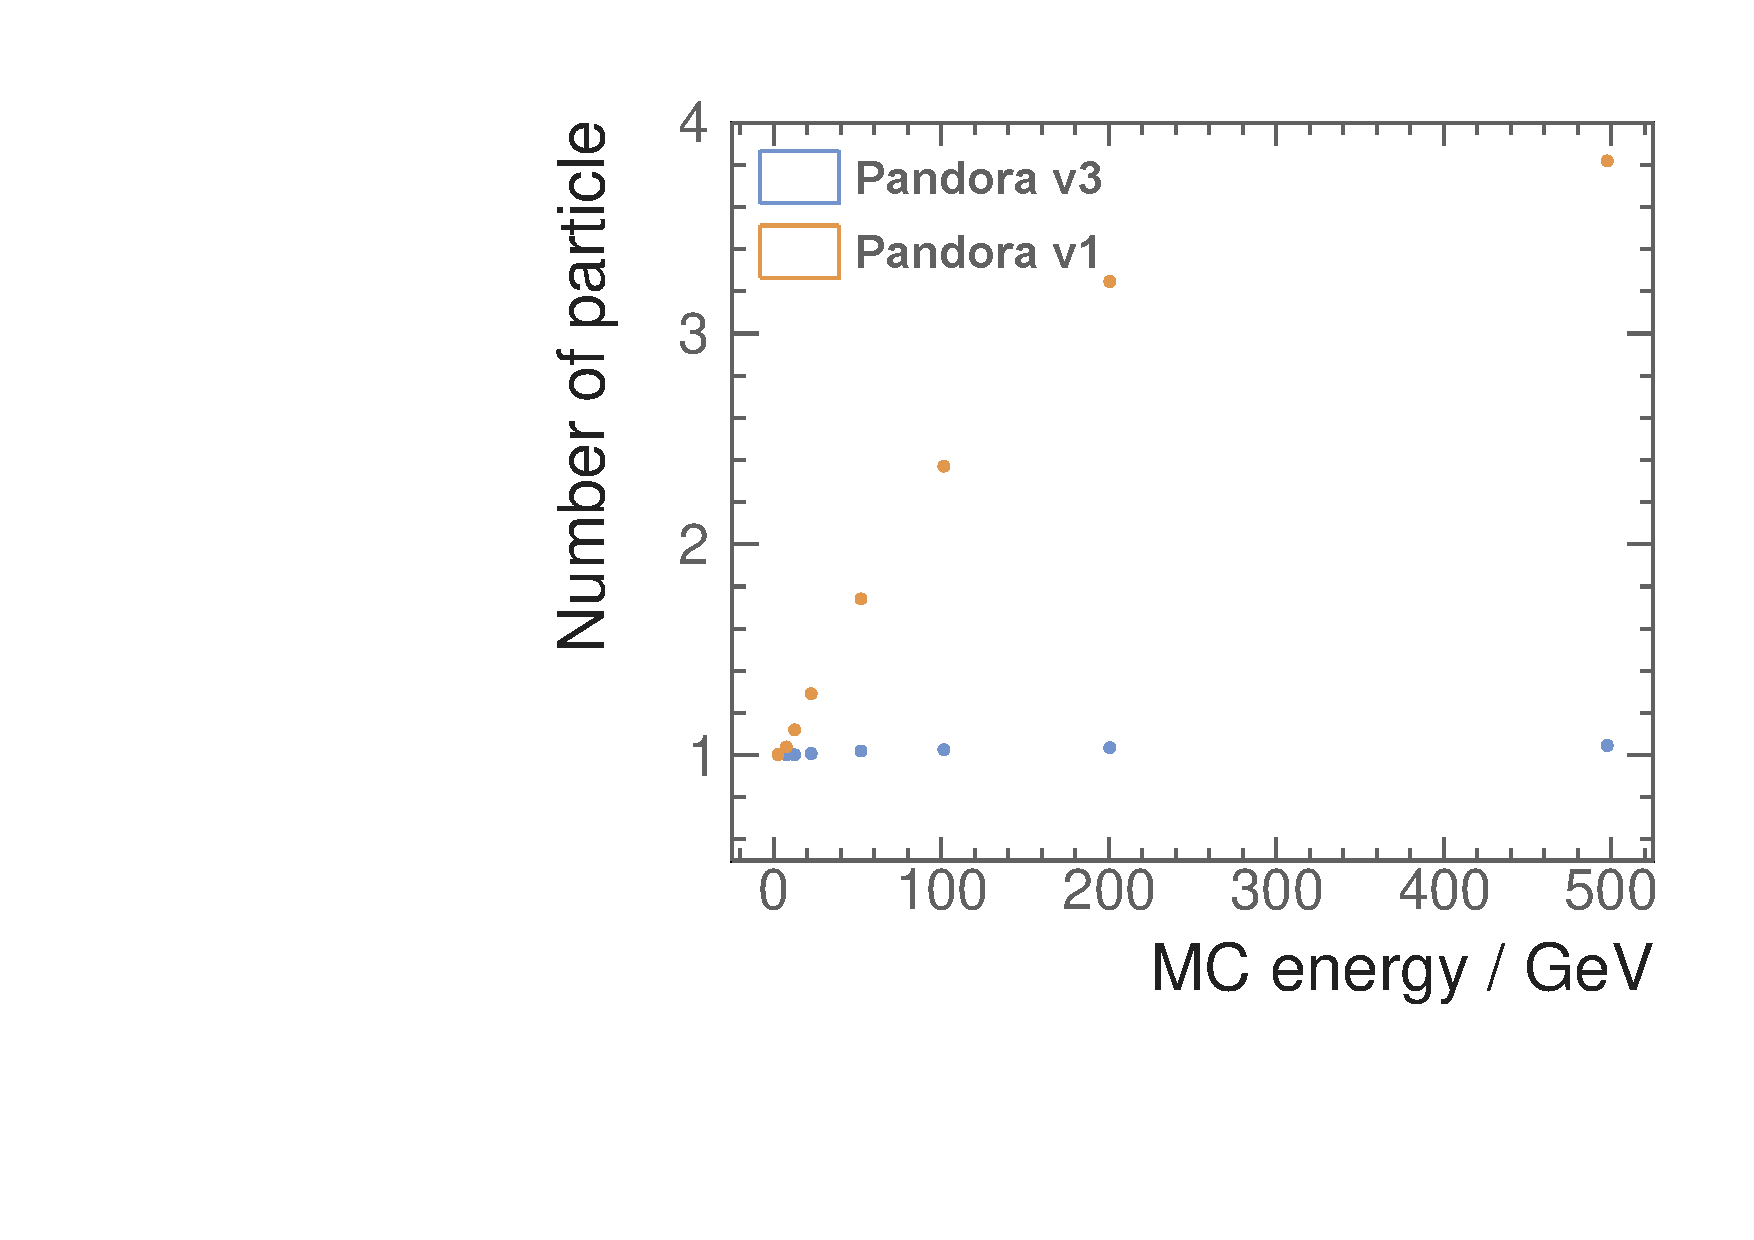
\includegraphics[width=\textwidth]{photon/SingleN_alledit.pdf}
        \caption{}
        \label{fig:photonSingleN_all}
    \end{subfigure}
\caption[Average number of reconstructed photons and reconstructed particles, as a function of their true energy using single photon sample.]
{Average number of reconstructed a) photons, and b) reconstructed particles, as a function of their true energy using a single photon per event sample. For both figures, the top orange and bottom blue dots are reconstructed with \pandora version 1 and version 3, respectively. The photon reconstruction is changed in \pandora version 2.}
\label{fig:photonSingleN}
\end{figure}

A similar trend of  reduction in the number of reconstructed particles is shown in \Figure{fig:photonSingleN_all}, where the extra fragments identified as neutral hadrons have also taken into account. For a 100\,GeV photon, the average number of particles is reduced to 1 2.4. For a 500\,GeV photon, the number is reduced to 1.05 from 3.8.


\FIGURE{fig:photonDoubleCompareN} illustrates a reduction in the photon fragments and the neutral hadron fragments using two photons of 500 and 50\,GeV per event sample. The figure shows the MC distance separation from 0 to 30\,mm, which corresponds to approximately 6 \ECAL square cells of the default \ILD detector model. This is a difficult test for fragment removal as high energy photons are more likely to create fragments and the imbalance in the two photon energies makes it more difficult to separate correctly.  In both \Figure{fig:photonDoubleCompareN_p} and \Figure{fig:photonDoubleCompareN_all}, the average numbers of photon and particle are below 2.05 at 30\,mm apart, which is significantly better than the reconstruction in \pandora version 1. Two photons start to be resolved at 10\,mm apart, and fully resolved at 20\,mm apart. The resolution is better than reconstruction in \pandora version 1, which is difficult to extract due to excess fragments.

\begin{figure}[tbph]
\centering
    \begin{subfigure}[b]{0.45\textwidth}
        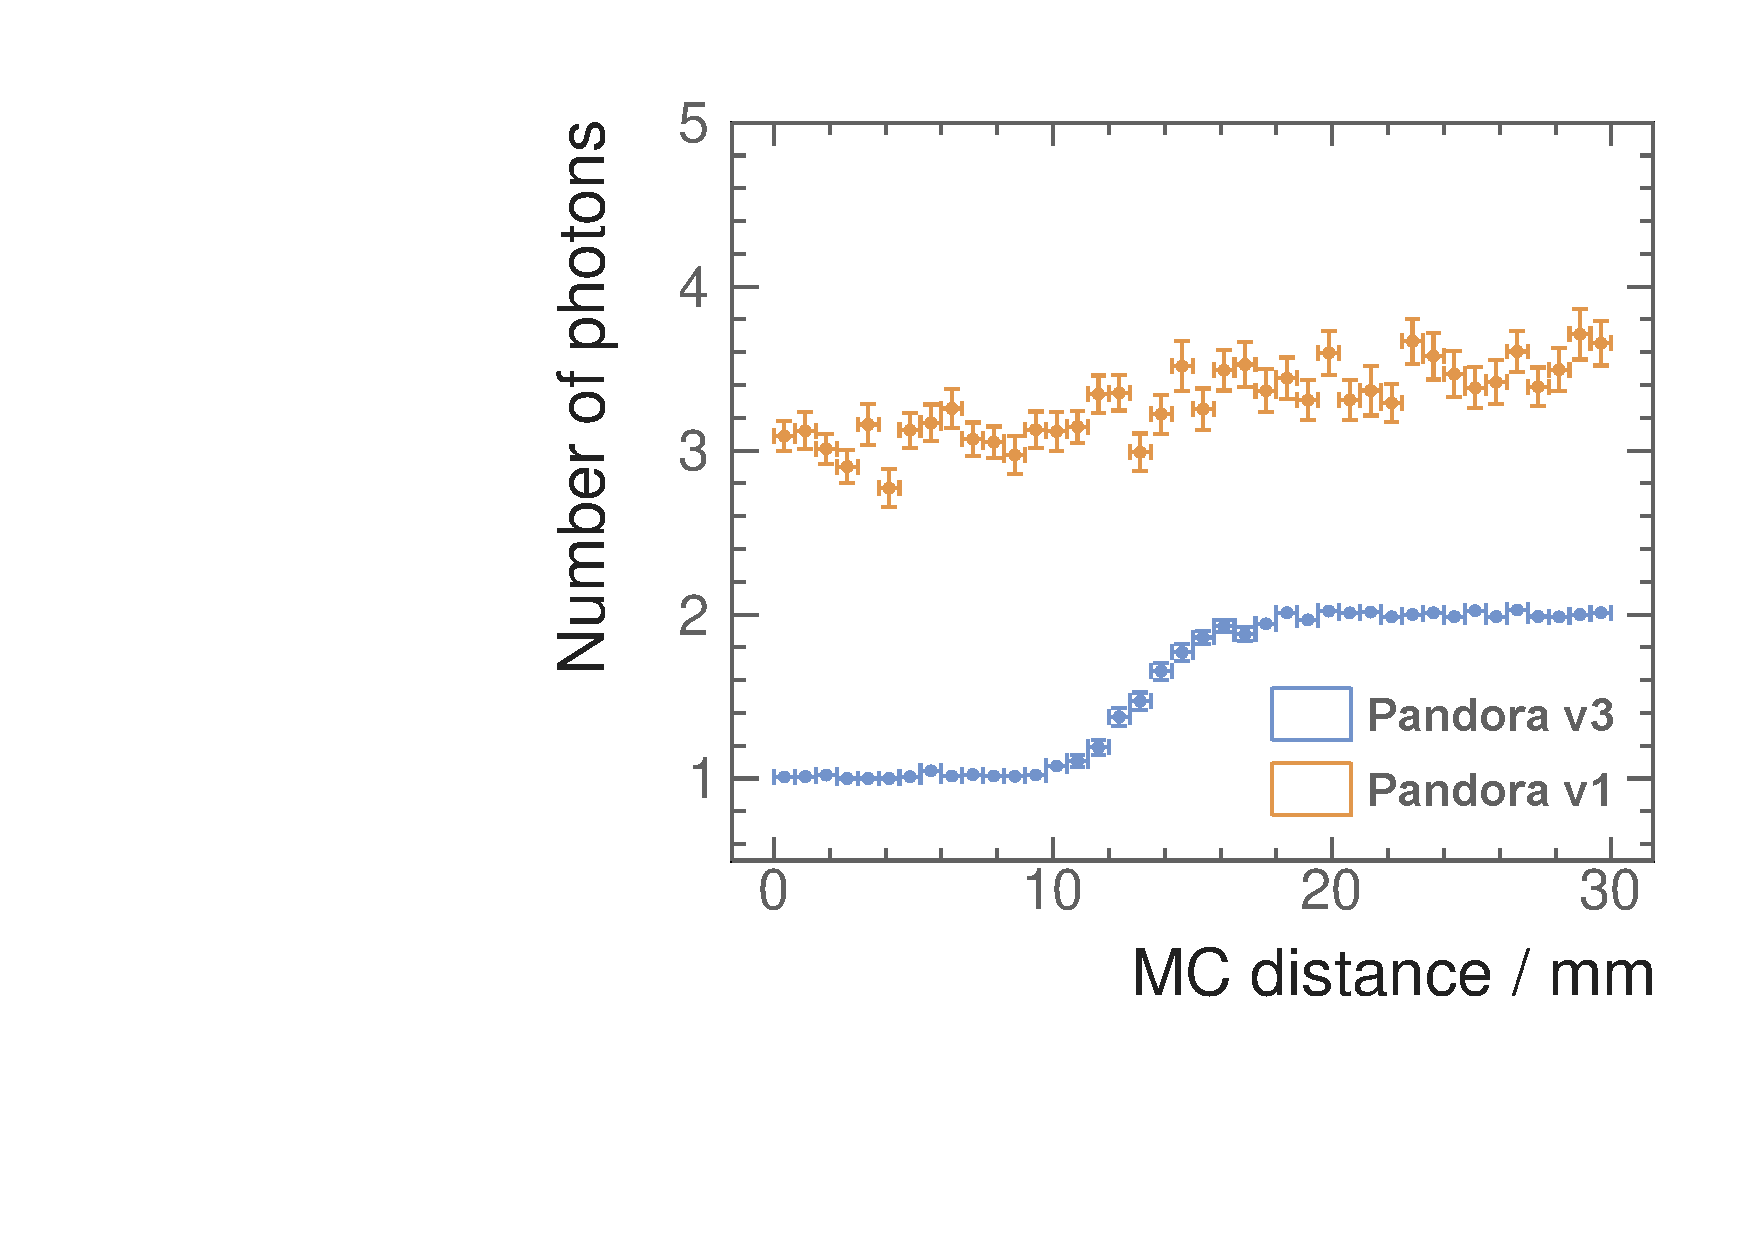
\includegraphics[width=\textwidth]{photon/DoubleCompareN_p3edit.pdf}
        \caption{}
        \label{fig:photonDoubleCompareN_p}
    \end{subfigure}
    \begin{subfigure}[b]{0.45\textwidth}
        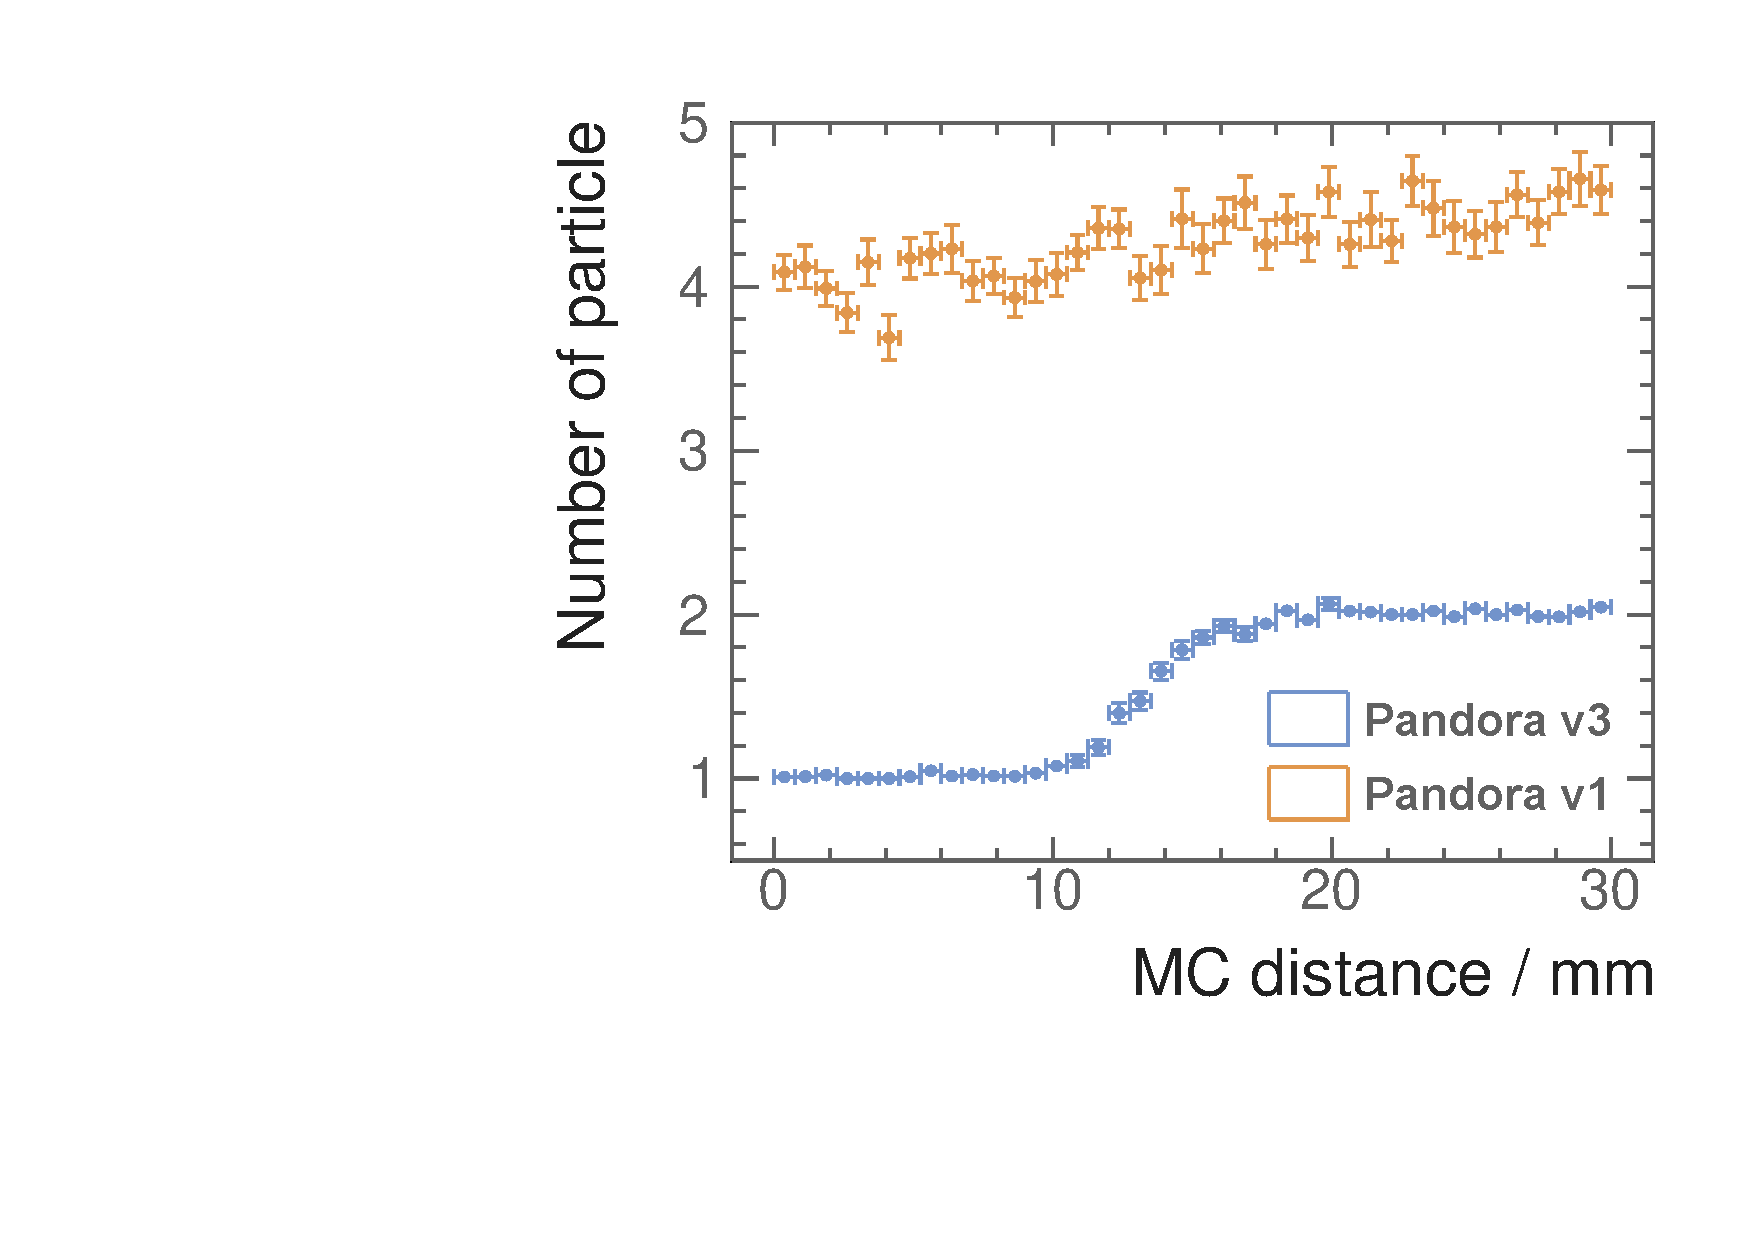
\includegraphics[width=\textwidth]{photon/DoubleCompareN_all2edit.pdf}
        \caption{}
        \label{fig:photonDoubleCompareN_all}
    \end{subfigure}
\caption[Average number of reconstructed photons and reconstructed particles, as a function of the MC distance separation.]
{Average number of reconstructed a) photons, and b) particles, as a function of the MC distance separation in the calorimeter, using two photons of 500 and 50\,GeV per event sample. For both figures, the top orange and bottom blue dots are reconstructed with \pandora version 1 and version 3, respectively. The photon reconstruction is changed in \pandora version 2.}
\label{fig:photonDoubleCompareN}
\end{figure}





Another metric to reflect the improvement in photon reconstruction is the fraction of the fragment energy to the total energy as function of the distance separation. Shown in \Figure{fig:photonDoubleFragEnergy}, using two photons of 500 and 50\,GeV per event sample, a reduction in fragment energy can be seen clearly. With improved reconstruction, the average fragment energy fraction is below 0.1\% up to 30\,mm apart, whilst around 5\% energy would be reconstructed in fragments with \pandora version 1.
\begin{figure}[tbph]
\centering
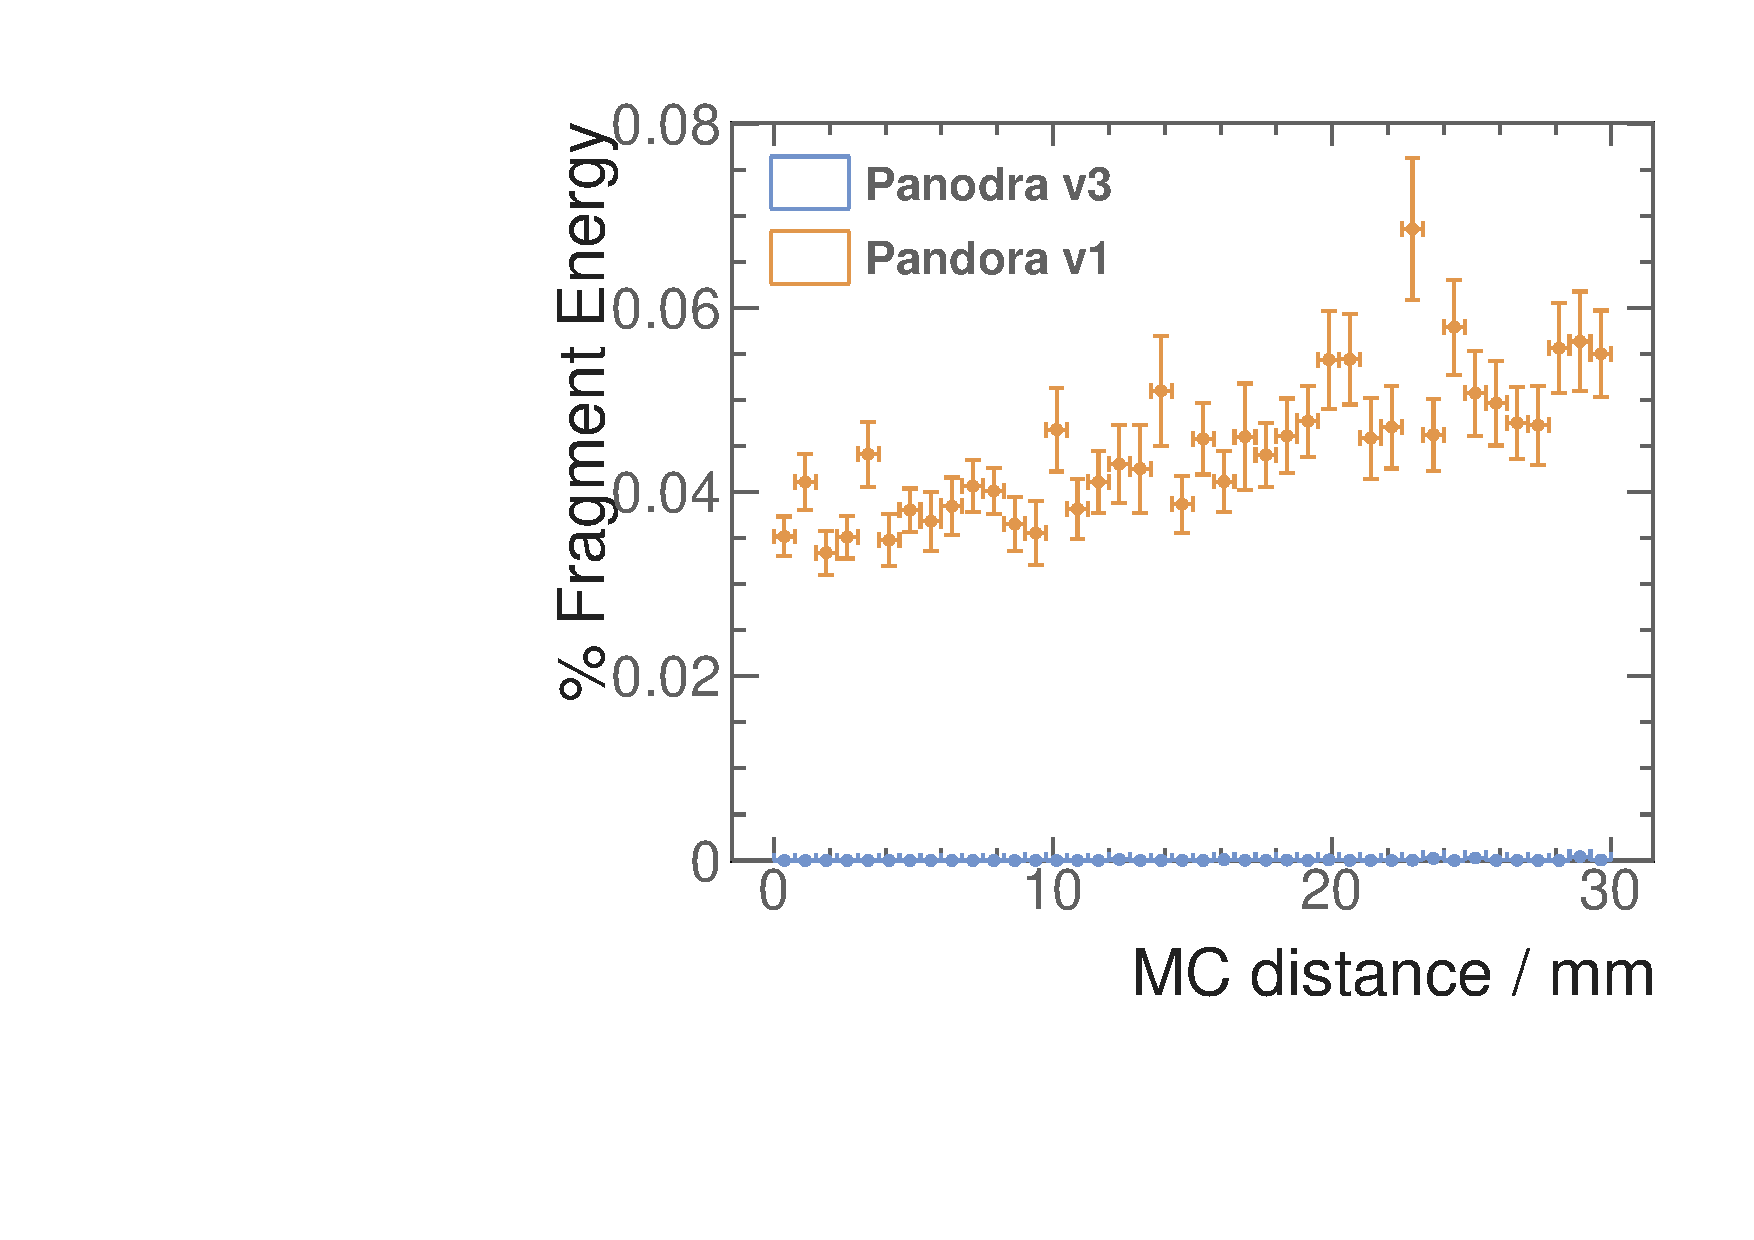
\includegraphics[width=0.45\textwidth]{photon/DoubleCompareFragEnergy.pdf}
\caption[Average fraction fragments energies of the total energy, as a function of the MC distance separation]
{Average fraction of fragments energies to the total energy, as a function of the MC distance separation in the calorimeter, using two photons of 500 and 50\,GeV per event sample. The top orange and bottom blue dots are reconstructed with \pandora version 1 and version 3 respectively. The photon reconstruction is changed in \pandora version 2.}
\label{fig:photonDoubleFragEnergy}
\end{figure}




The improvement in completeness and resolution in photon reconstruction, as shown in single photon and double photon reconstruction, leads to a small improvement in the jet energy resolution at high energy. The total jet energy is sampled at 91, 200, 360 and 500\,GeV. Shown in \Figure{fig:photonJER}, the jet energy resolutions are better at 360 and 500\,GeV with improved photon reconstruction. This is due to more aggressive photon reconstruction especially nearby tracks, which is more useful at a high-energy dense jet environment.



The improvement of the photon is also demonstrated in \Chapter{chap:Tau}, where tau lepton decay modes are classified. Excellent photon reconstruction leads to a high classification rate.

\begin{figure}[tbph]
\centering
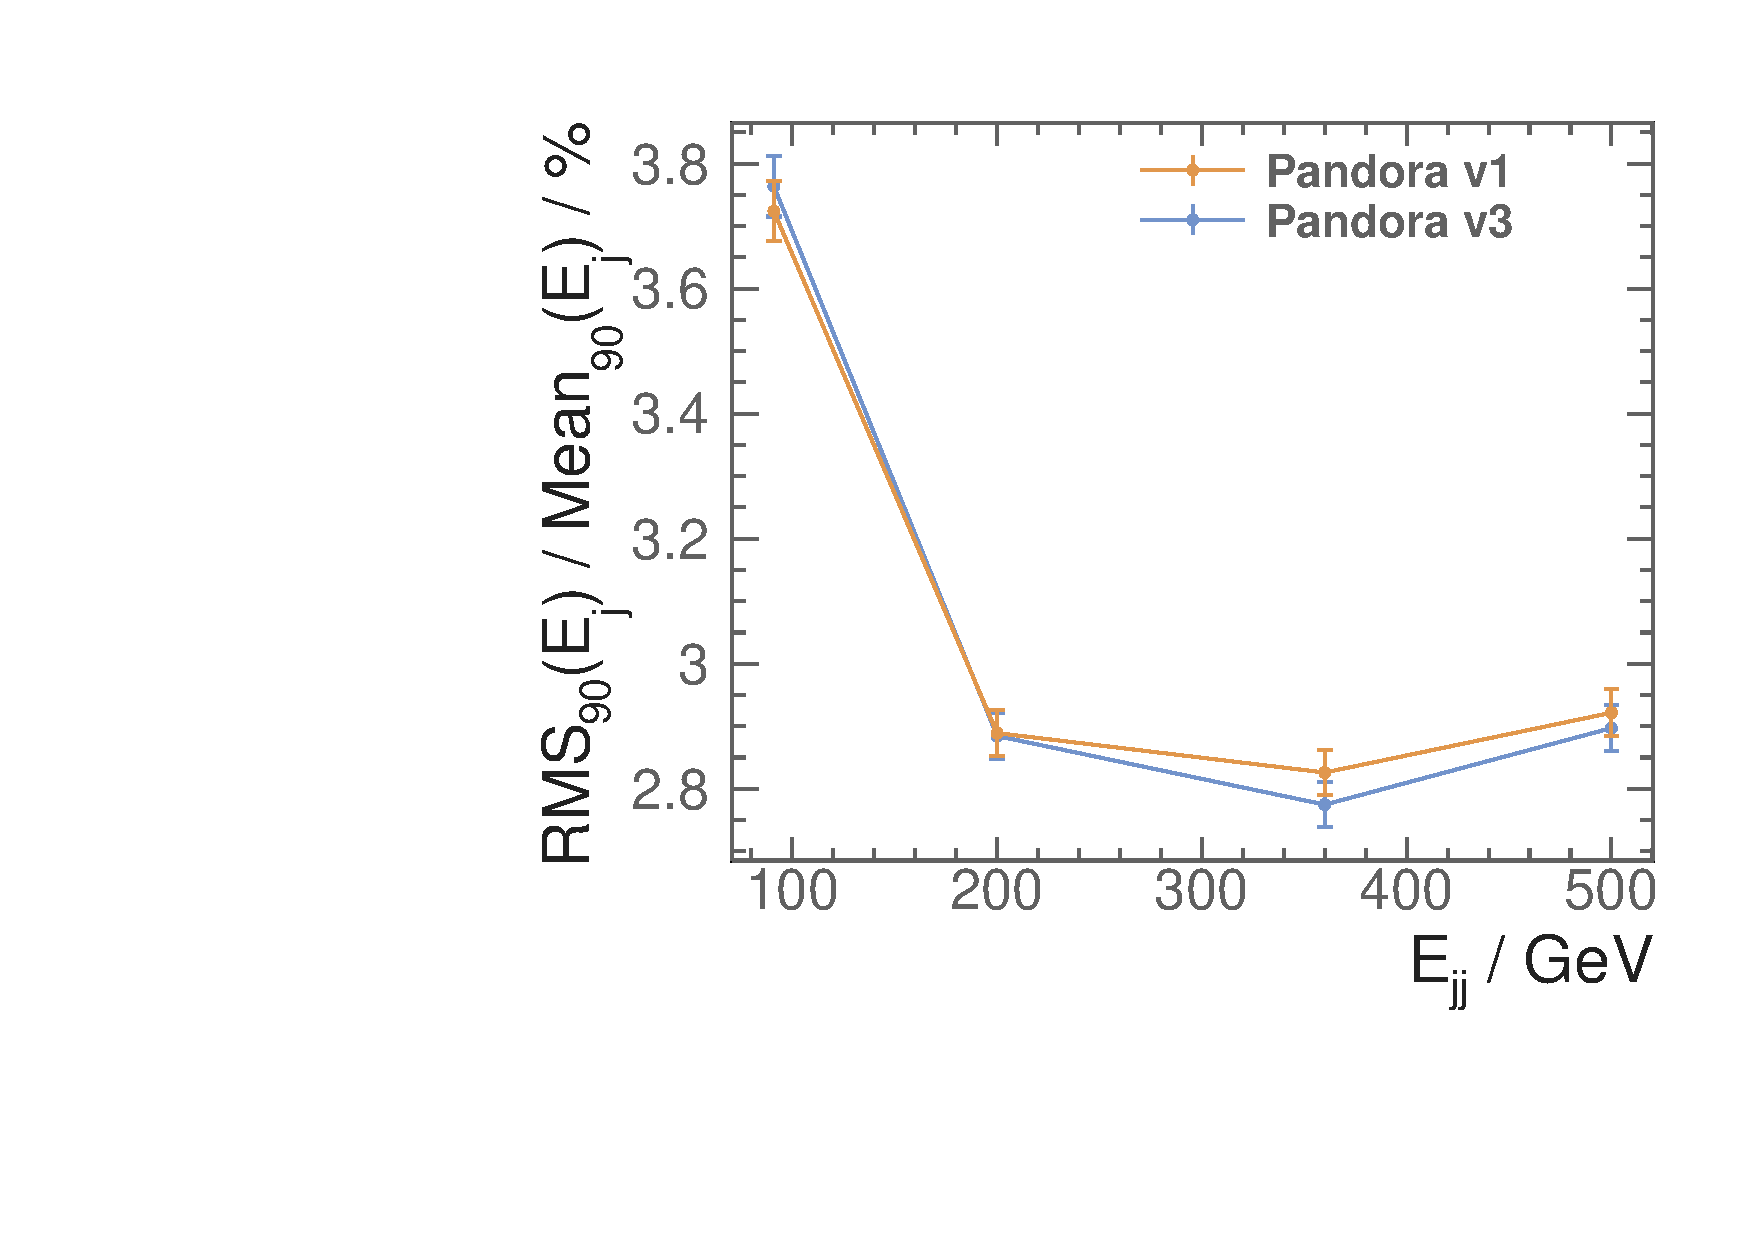
\includegraphics[width=0.45\textwidth]{photon/JERnew.pdf}
\caption[Jet energy resolution as a function of the di-jet energy]
{Jet energy resolution as a function of the total jet energy using \Zuds sample at barrel region. The top orange and bottom blue dots are reconstructed with \pandora version 1 and version 3. The photon reconstruction is changed in \pandora version 2.}
\label{fig:photonJER}
\end{figure}


\section{Understand photon reconstruction improvement}




%As stated before, the photon reconstruction algorithm in \Section{sec:photonRecostrcution} and the photon splitting algorithm in \Section{sec:photonSplitting}  improves the photon completeness and the photon pair resolution. The fragment removal algorithm in \Section{sec:photonFragRemoval} removes fragments in the \ECAL. High energy fragment removal algorithm in \Section{sec:photonHighEFragRemoval} removes fragments in the \HCAL.

To show the incremental improvement of individual algorithm, the average number of particle for a high energy photon pair, 500 - 500\,GeV is shown in \Figure{fig:photonDoubleCompareAlgs}. Blue, orange, and green dots represent full photon reconstruction, only fragment removal algorithms in the \ECAL, and fragment removal algorithms in the \ECAL and the \HCAL, respectively.

With fragment removal algorithm in the \ECAL, the number of fragment is reduced significantly (comparing with \Figure{fig:photonDoubleCompareN_all}). With the additional fragment removal in the \HCAL, the number of fragments are reduced further. At 40\,mm apart, with both fragment removal algorithms (green dots), there is less than 0.05 fragment per photon pair.

The introduction of the revised photon reconstruction and photon splitting improves the photon separation resolution. Photons pair starts to be resolved at 5\,mm apart for 500 - 500\,GeV pair and fully resolved at 15\,mm apart. With previous photon reconstruction in \pandora version 1, the same photon pair starts to be resolved at 10\,mm apart and fully resolved at around 40\,mm apart.


\begin{figure}[tbph]
\centering
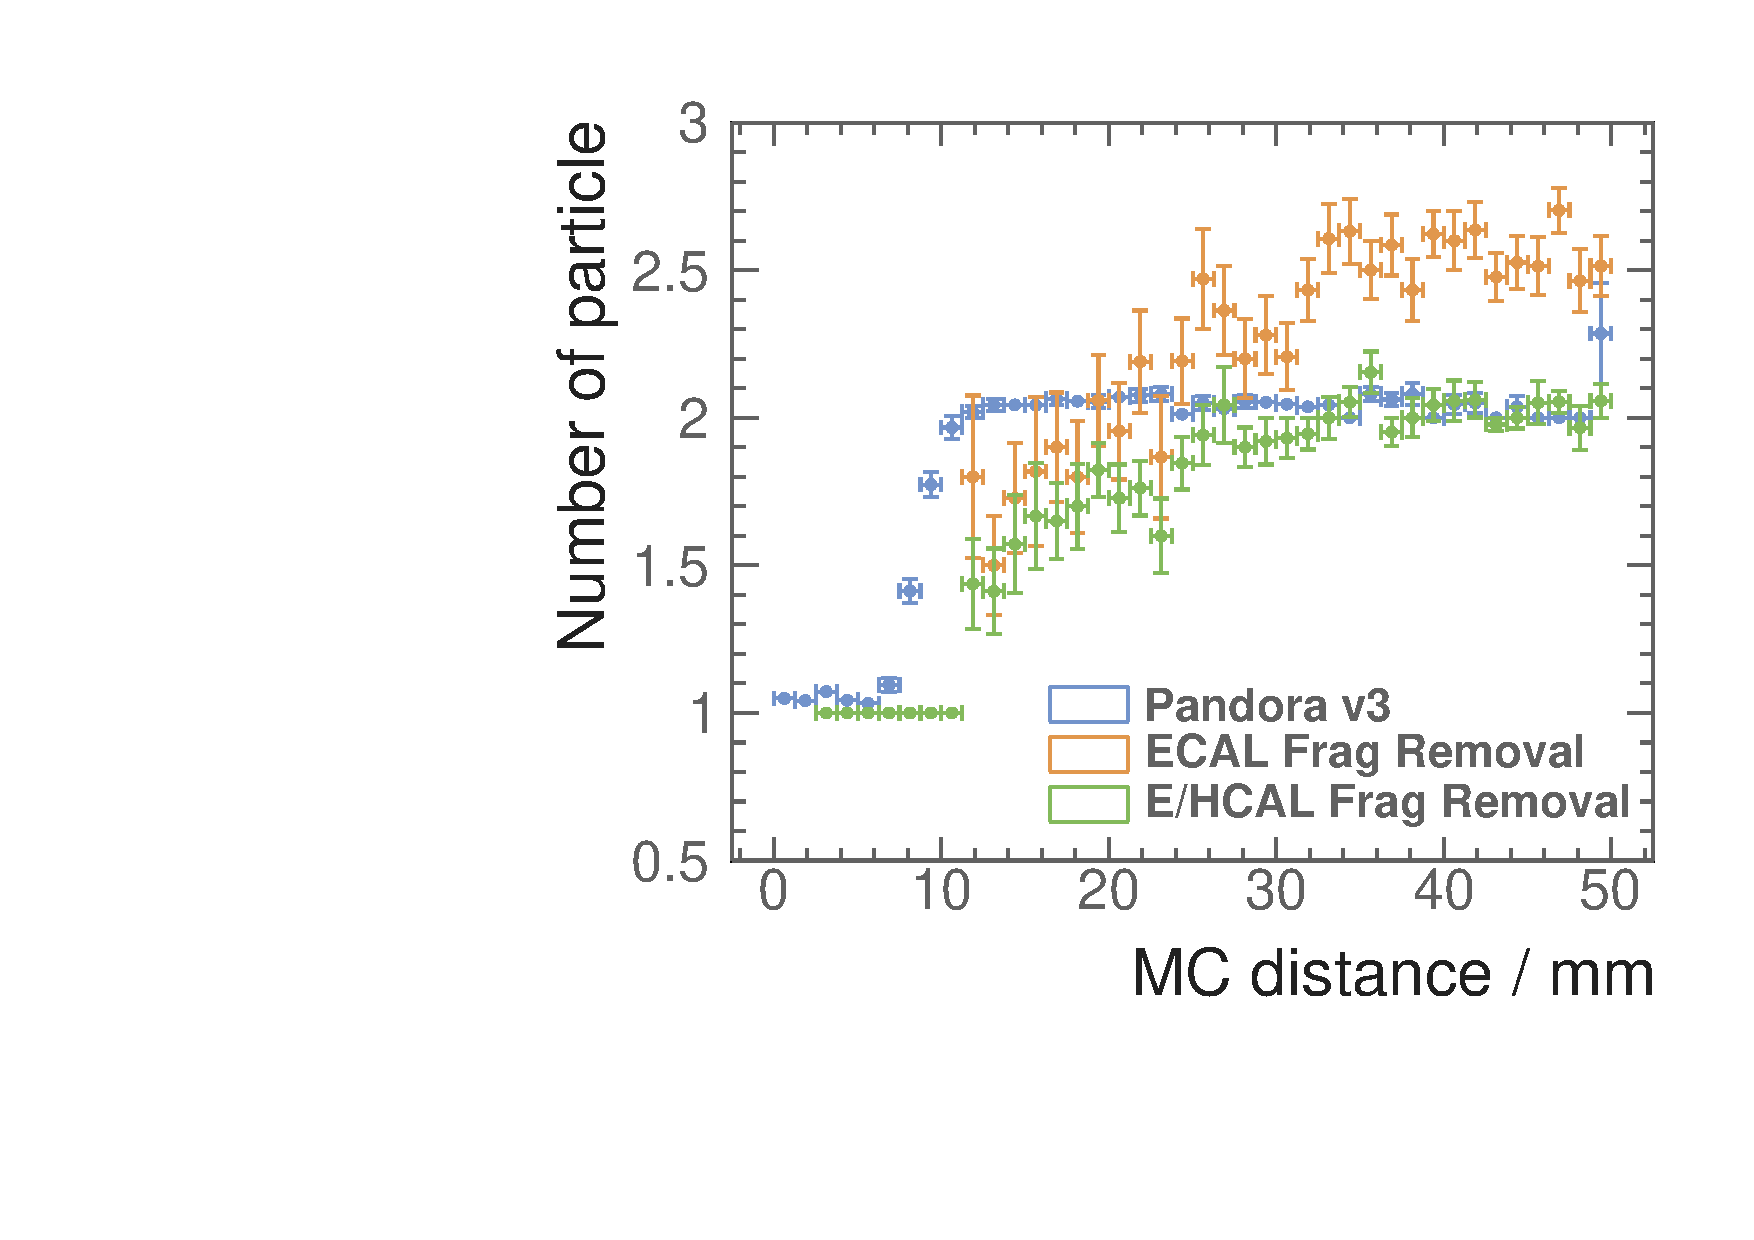
\includegraphics[width=0.45\textwidth]{photon/DoubleCompareAlgs.pdf}
\caption[Average number of photons, as a function of the MC distance separation for different algorithms combinations.]
{Figure shows the average number of photons, as a function of the MC distance separation in the calorimeter, using two photons of 500 and 500\,GeV per event sample. The blue, orange, and green dots are reconstructed with \pandora version 3, \pandora version 1 with fragment removal in the \ECAL, and \pandora version 1 with fragment removal in the \ECAL and the \HCAL. The photon reconstruction is changed in \pandora version 2.}
\label{fig:photonDoubleCompareAlgs}
\end{figure}

\section{Current photon reconstruction performance}

In \Section{sec:photonPerformanceCompare}, the improved performance of the photon reconstruction is demonstrated with different metrics, using single photon, double photons and jet samples. In this section, the performance of the photon reconstruction as a function of photon energies will be described.


Single particle reconstruction and ID efficiency is demonstrated in \Figure{fig:photonSingleEffPerformance}. Using single photon samples, an event can have an efficiency of 1, if the photon reconstructed corresponds to the truth photon, or an efficiency of 0. The low efficiency in the first bin, from 0 to 0.25\,GeV is because photon reconstruction does not attempt to reconstruct photons below 0.2\,GeV.  The single photon reconstruction efficiency is above 98\% for photons above 2\GeV and above 99.5\% for photons above 100\,GeV.

\begin{figure}[tbph]
\centering
    \begin{subfigure}[b]{0.45\textwidth}
        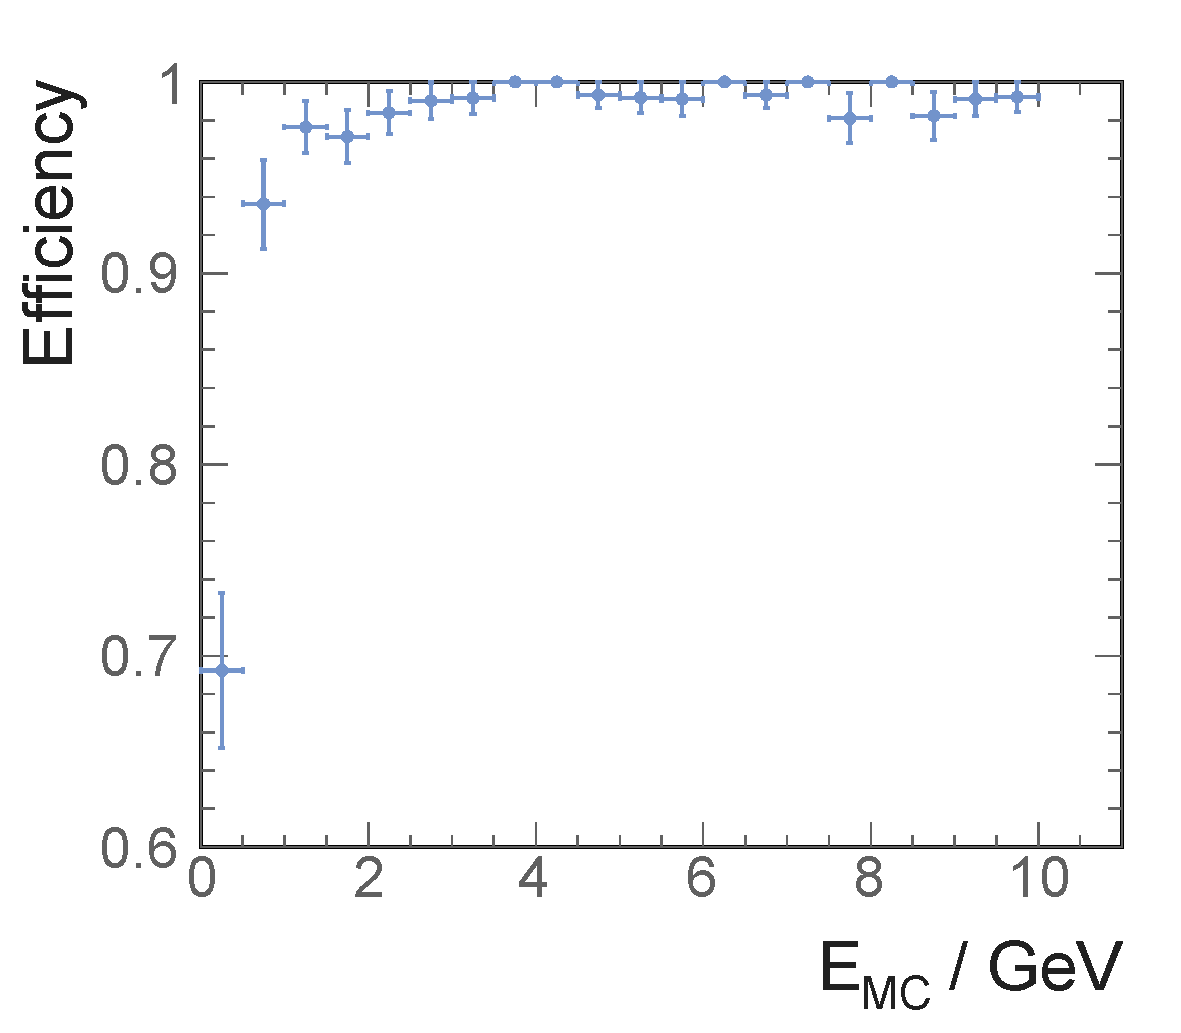
\includegraphics[width=\textwidth]{photon/singlePhotonEff2fullEdt}
        \caption{}
        \label{fig:photonSingleEffLow}
    \end{subfigure}
    \begin{subfigure}[b]{0.45\textwidth}
        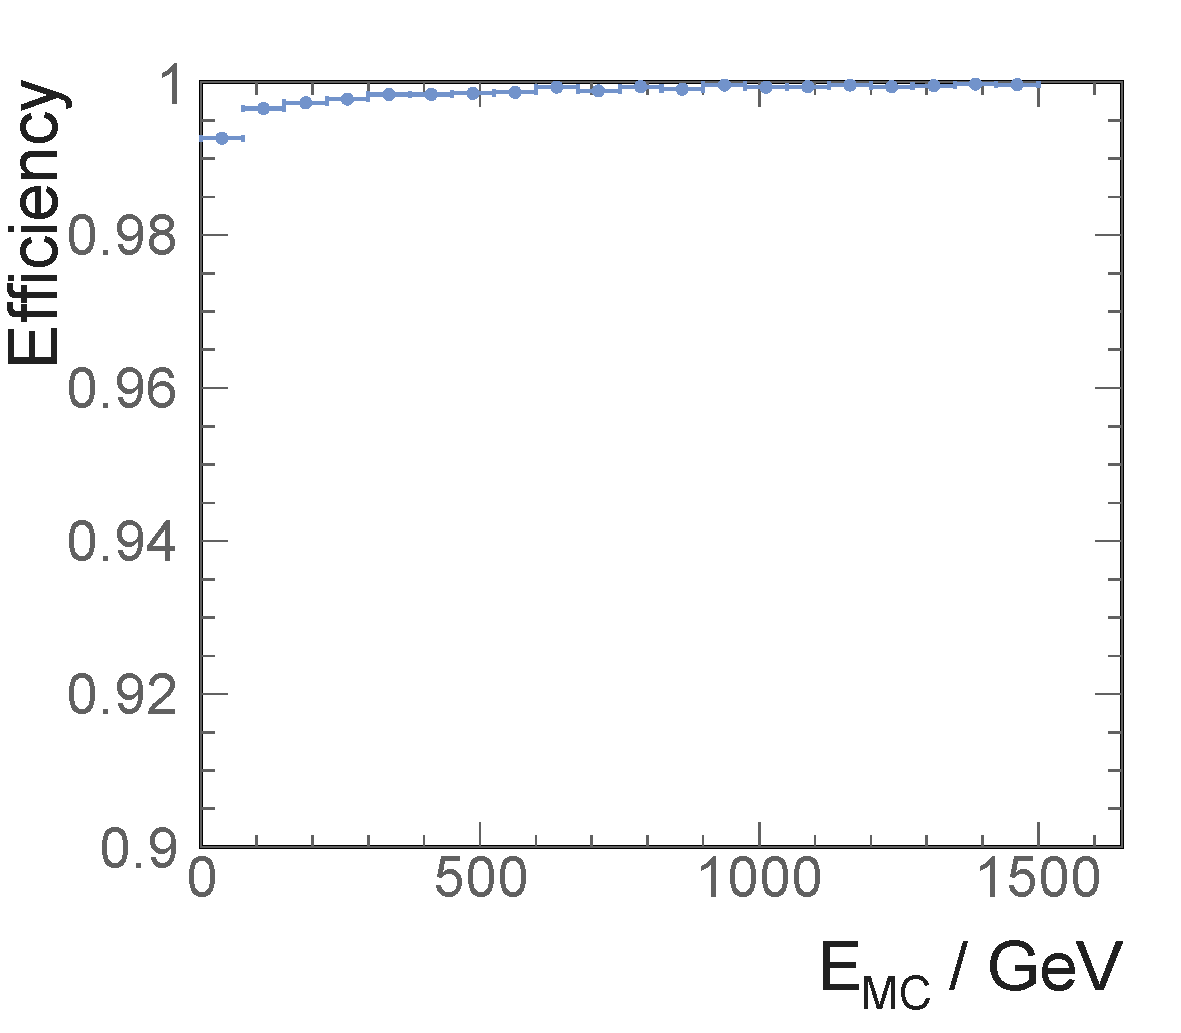
\includegraphics[width=\textwidth]{photon/singlePhotonEffEdt}
        \caption{}
        \label{fig:photonSingleEff}
    \end{subfigure}
\caption[Single photon reconstruction efficiency as a function of energy.]
{Single photon reconstruction efficiency as a function of energy. \FIGURE{fig:photonSingleEffLow} shows the low energy region and \Figure{fig:photonSingleEff} shows high energy region.}
\label{fig:photonSingleEffPerformance}
\end{figure}



For simple samples such as two photons per event, there are very few fragments. Shown in \Figure{fig:photonDoubleCompareN_pN_all} for 500 and 50\,GeV photons pair sample, the average number of photons and particles beyond 20\,mm apart is less than 0.05 above the true value, 2.

\begin{figure}[tbph]
\centering
        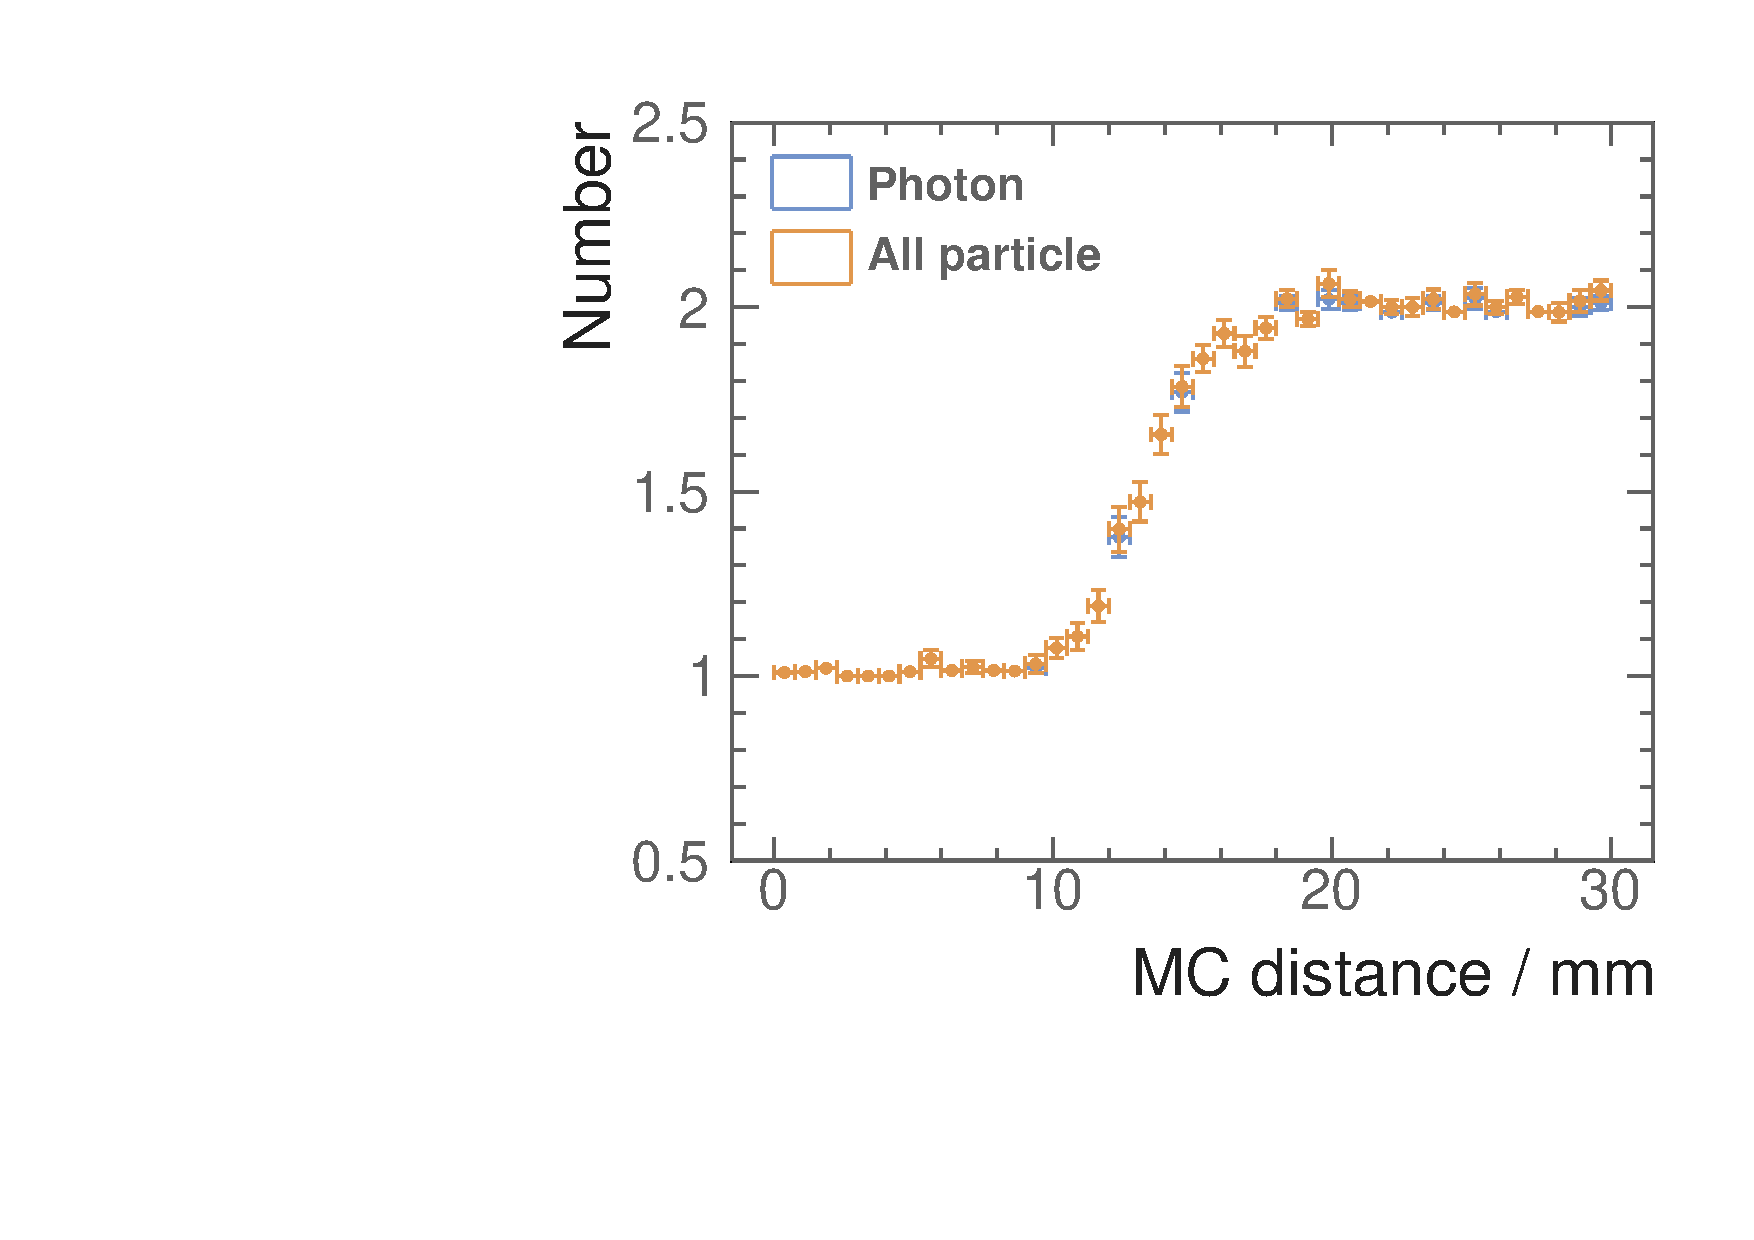
\includegraphics[width=0.85\textwidth]{photon/DoubleN_pN_all.pdf}
        \caption{Average numbers of photon  (blue) and particle (orange) using two photons of 500 and 50\,GeV per event sample. }
        \label{fig:photonDoubleCompareN_pN_all}
\end{figure}

The resolving power of a photon pair depends on energies of two photons. \FIGURE{fig:photonDoubleCompareEnergies} is an example of average number of photon reconstructed for differen photon pairs. When the energies of two photons are similar, the resolving power is greater. This is because that the two photon showers have similar sizes, and the \peakFinding algorithm can exploit the symmetry in the size of the EM showers. For example, 500 - 500\,GeV photon pair and 10 - 10\,GeV photon pair start to be resolved at 6\,mm apart, which is about 1 \ECAL cell. The asymmetrical photon pair,  500 - 50\,GeV and  100 - 10\,GeV pair, starts to be resolved at 10\,mm apart, which is about 2 \ECAL cells.

For an energetic photon, it is more difficult to remove fragments, but it is easier to identify the photon. The electromagnetic shower core is more dominant than the peripherals. Therefore separating two energetic photons is easier than separating two low energy photons. This can be seen in \Figure{fig:photonDoubleCompareEnergies}. At 20\,mm apart, two photons in  500 - 500\,GeV pair are fully resolved, where approximately only 60\% of two photons in 10 - 10\,GeV pair are resolved.

\begin{figure}[tbph]
\centering
        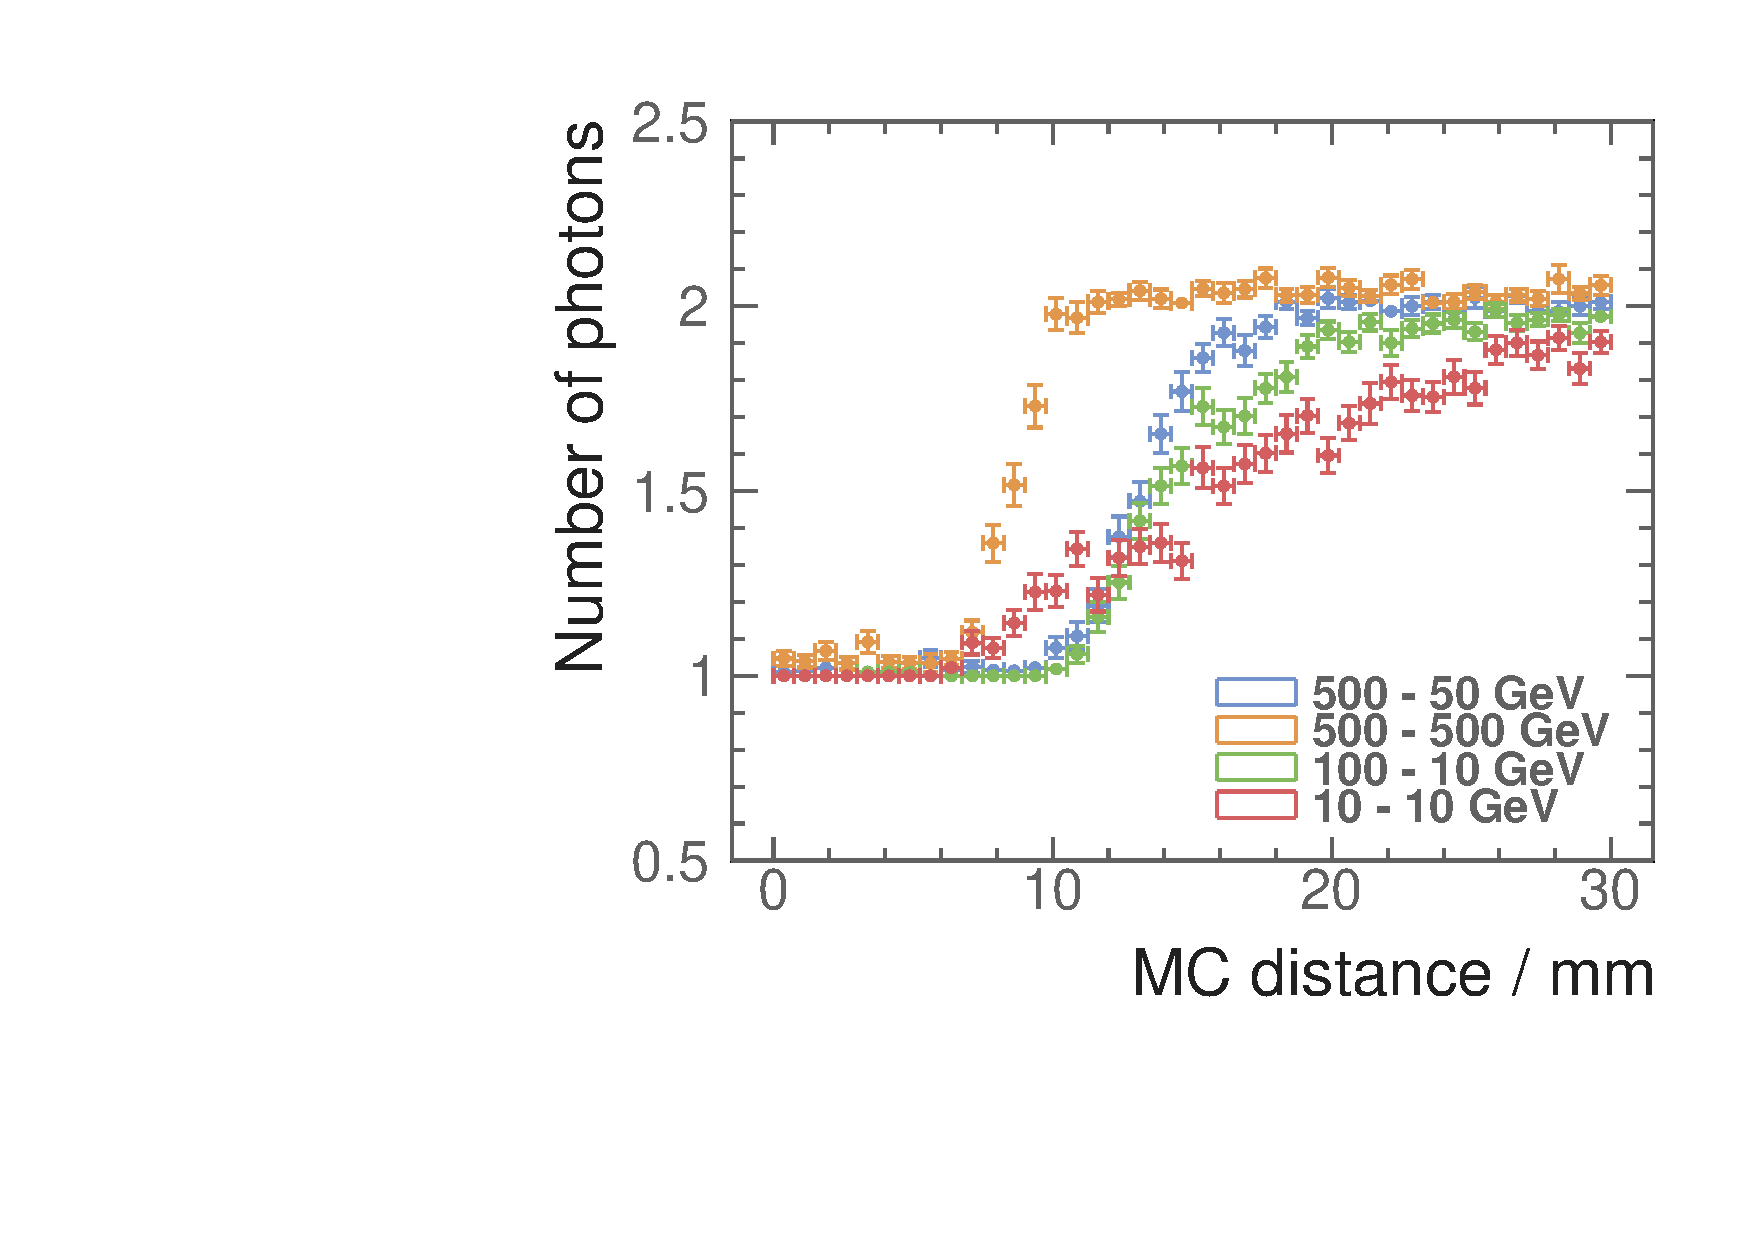
\includegraphics[width=0.85\textwidth]{photon/DoubleCompareEnergies.pdf}
        \caption{Average numbers of photon for four different photon pairs: 500 - 50 (blue), 500 - 500 (orange), 100 - 10 (green), and 10 - 10\,GeV (red).}
        \label{fig:photonDoubleCompareEnergies}
\end{figure}

